\documentclass[10pt]{article}
\usepackage[final]{graphicx}
\usepackage{amsfonts}

\usepackage{float}
\usepackage{subfig}
\usepackage{natbib}


% lasith added 
\usepackage{amsmath, amsthm}
\usepackage{url}

\topmargin-.5in
\textwidth6.6in
\textheight9in
\oddsidemargin0in

\def\ds{\displaystyle}
\def\d{\partial}

%below packages are for algorithm
\usepackage{algorithm}
\usepackage[noend]{algpseudocode}

\makeatletter
\def\BState{\State\hskip-\ALG@thistlm}
\makeatother 
%above packages are for algorithm



\begin{document}

\centerline{\large \bf Title of Report}

\vspace{.1truein}

\def\thefootnote{\arabic{footnote}}
\begin{center}
  Author 1\footnote{Department, University},
  Author 2\footnote{Department, University},
  Author 3\footnote{Department, University},
  Author 4\footnote{Department, University},
  Author 5\footnote{Department, University}
\end{center}

%\vspace{.1truein}

\begin{center}
Faculty Mentors: Mentor 1\footnote{Company},
Mentor 2\footnote{University}
\end{center}


\vspace{.3truein}
\centerline{\bf Abstract}

Tracking coastal bathymetry is necessary for marine navigation, military activities, and assessment of storm damage as beaches evolve. Past efforts have derived surface wave properties from in situ bathymetric measurements. However, in situ measurements are costly and laborious to collect. As a result, direct observations of bathymetry are sparse in time and space. On the other hand, remotely sensed observations of surface conditions are becoming easier to obtain. We seek methods to invert for bathymetry given surface conditions. 

We utilize linearized wave theory to estimate bathymetry near Duck, NC given measurements of surface wave properties collected by the U.S. Army Corps of Engineers. We process measurements of wave height, wave number, and bathymetry for easy incorporation into and validation of models. We also create a forward model to estimate wave number and wave height given bathymetry information. Several inverse methods including nonlinear least squares, Markov Chain Monte Carlo, and Tikhonov regularization then employ the data and forward model to estimate bathymetry along a one-dimensional profile.

Our results demonstrate good estimates of depth, $h$, in the near shore region, within $500~m$ of the beach. All inverse methods are able to accurately reconstruct a sandbar located in this region which is an important feature for consideration of rip tides and coastal navigation. Accuracy of the methods drops off past $\sim550~m$ from shore due to the increased depth and subsequent lower sensitivity of wave number to depth. We suggest several avenues for possible expansion of this work in the future which may improve overall accuracy of depth estimates.

\section{Introduction}
Bathymetry is a measurement of submarine topography and can be used to understand shifts of the ocean floor and its depth. Knowledge of bathymetry is important for marine navigation, both civilian and military, as well as for monitoring and predicting the effects of storms on coastal environments. While direct measurement of bathymetry is possible, the process tends to be cost and time prohibitive. For example, amphibious vehicles are capable of spatially limited surveys of bathymetry in difficult surf-zone conditions but require significant resources to operate. As a result of these factors, surveys tend to be sparse in time. 

The research we conducted for this report focuses on a method to estimate bathymetry, using surface measurements collected via remote sensing platforms, i.e. airborne, satellite, or onshore platforms. While bathymetry data is currently sparse due to observational limitations, the physics of waves are reasonably well understood. In particular, a dispersion relationship can be used to relate water depth to surface properties such as wave length and wave period. This relationship makes it possible to estimate bathymetry given the observations of these parameters. Light Detection And Ranging (LiDAR) has been used to determine wave heights and Argus land-mounted video has been analyzed photogrammetrically to determine wave frequency and wave number. Moreover, these resources  provide valuable inputs for estimating coastal bathymetry in a more efficient manner than is currently available.

Wave and bathymetric data has been collected in Duck, NC by the U.S. Army Corps of Engineers Coastal and Hydraulics Laboratory, including in situ measurements of bathymetry and measurements of the water surface. These measurements provide a method for testing algorithms to invert for bathymetry because the true bathymetry is available for comparison to the numerical estimates.

We invert for depth, \textit{h}, using wave number with a 1D model derived using the energy flux method to create a correlation between wave length and depth from the water surface as shown in Figure~\ref{flowchart}.
\begin{figure}[H]
		\centering
		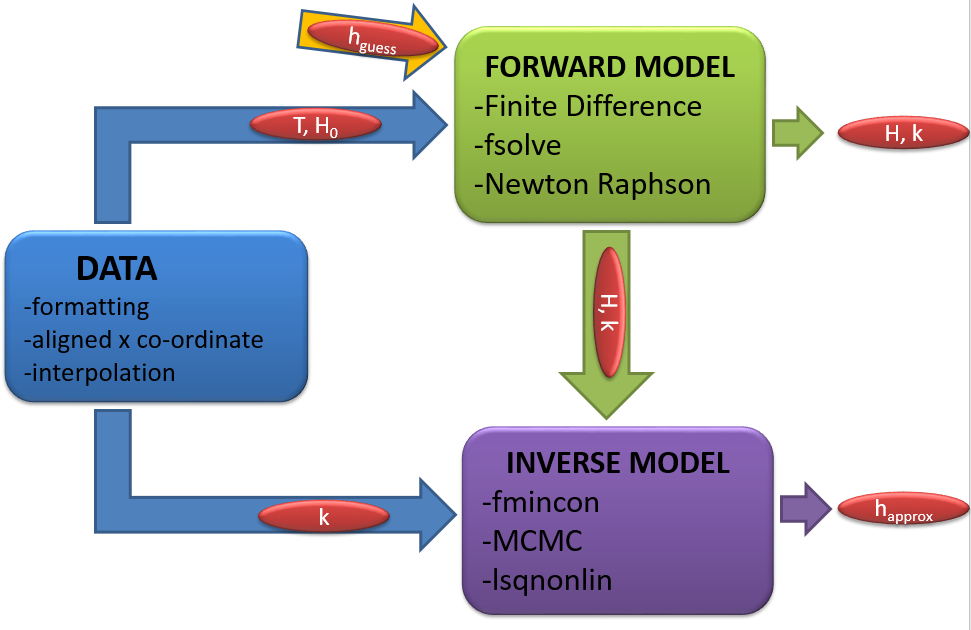
\includegraphics[width=.90\linewidth]{img/Flow_Chart.png}
		\caption{Flow chart of the workflow for this research}
		\label{AWAC}
\end{figure}
In section 2 we discuss about how data is observed and use to measure different wave parameters. In section 3 we discuss about the forward problem and numerical results of forward problem. Inversion method is discussed in section 4 with discussion related the methods applied. In the last section 5 we discuss about the experimental results. These results were generated using both simulated and real data using some existing tools.

\section{The Problem}
%==============================================

Although there have been uncertainties in capturing the topography of the ocean near shore, mathematical methods can estimate bathymetry using the dispersion relationship between wavelength and the period. Stockdon et al. used video imagery, which compared true wave signal and remotely sensed video signal to create a linear representation between wave amplitudes and phases \citep{stockdon2000}.  Holman et al. used a 2-dimensional method with Kalman filtering to estimate the depth, $h$ \citep{holman2013}.

We invert for depth, \textit{h}, using wave length and wave number with a 1D model derived using the energy flux method to create a correlation between wave length and depth from the water surface as shown in Figure~\ref{flowchart}.

\begin{figure}[h]
		\centering
		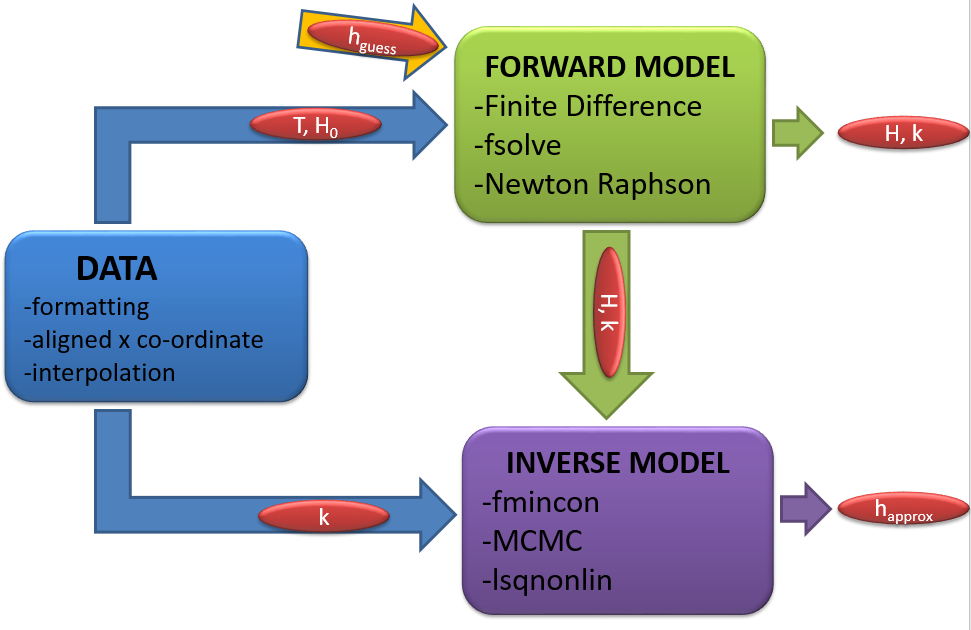
\includegraphics[width=.40\linewidth]{img/Flow_Chart.png}
		\caption{Flow chart of the workflow for this research}
		\label{AWAC}
\end{figure}

\subsection{Forward Problem}\label{forwardproblem}
The forward problem is described by 1D linear wave theory:
\begin{eqnarray}
\label{fp1}
\left \{
\begin{array}{lll}
\frac{d}{dx}\left(EC_g\right)=-\delta,\\
\\
\sigma^2=gk\tanh(kh),
\label{ode}
\end{array}
\right.
\end{eqnarray}
where $\delta$ is  wave breaking parameter and the speed at which the energy is transmitted, $C_g$, called linear theory group speed, is given as
\begin{equation}
\label{cg}
C_g=\frac{c}{2}\left(1+\frac{2kh}{\sinh(2kh)}\right),
\end{equation}
with $c=\frac{\sigma}{k}$ and from the linear theory, the wave energy, $E$ is given as
\begin{equation}
\label{e}
E=\frac{1}{8}\rho g H^2,
\end{equation}
$\rho$ is the density of water, $g$ is the gravitational acceleration, $\sigma$ is the angular frequency, $c$ is the local wave phase speed, $k$ is the wave number, $h$ is the water depth and $H$ is the wave height. Here, we assume $T$, the wave period, is constant.\\ 

\noindent Observe that equation \ref{fp1} is coupled using the fact that $\sigma=\frac{2\pi}{T}$. Hence, using equation \ref{cg} and \ref{e} in \ref{fp1}, we obtain
\begin{equation}
\label{fpdelta}
\frac{d}{dx}\left( \frac{\lambda}{k}\left(1+\frac{2kh}{\sinh(2kh)}\right)H^2 \right)=-\delta,
\end{equation}  
and 
\begin{equation}
\label{fk}
f(k) = gk\tanh(kh)-\sigma^2,
\end{equation}
where $k$ is the zero of function $f$ and $\lambda=\frac{\rho g \pi}{8T}$.\\

The wave breaking function, $\delta$, proposed by (Janssen and Battjes, 2007) is given as
\begin{equation}
\delta = \frac{1}{4h}B\rho g f H_{rms}^3\left[(R^3+\frac{3}{2}R)exp(-R^2)+\frac{3}{4}\sqrt{\pi}(1-erf(R))\right],
\end{equation}
This breaking function is basically depends on the wave height ${H}$ using the following parameters in terms of ${H}$\\
$$R=\frac{H_b}{H_{rms}}, \quad H_{rms} = 0.7H,\quad H_b=0.78h,\quad f=\frac{1}{T},\quad B=1.$$
In the above expression ${H_{b}}$ is the local wave breaking height, ${H_{rms}}$ is the root mean square of height and ${f}$ represents frequency. We can see that ${R}$ is wave breaking condition is provided 

\subsection{Numerical Solution of the Forward Model}
A finite difference scheme is applied to obtain a numerical solution with appropriate initial and boundary conditions. In the scheme of finite differences, the derivatives are replaced using their finite-difference approximations. The goal is to provide wave height using the finite difference method. In the process, MATLAB's fsolve function is applied to obtain the wave number. Furthermore, the Newton-Raphson method is used to verify the solution of wave number $k$ obtained by the fsolve function.
\subsubsection{Discretization of the Model}
A forward difference method is applied depending on the nature of the model given in equation (\ref{fpdelta}). The main goal is to obtain the wave height${H}$. In the process we calculate the following terms.\\
Total energy per unit area
$${E=\frac{1}{8}\rho g H_{rms}^2}$$\\
where ${\rho}$ is water density 1000${kg/m^3}$ and ${g}$ represents the gravitational acceleration ${9.8m/sec^2}$. \\
The root mean square of height as\\
$${H_{rms}=0.7 H}$$\\
Group wave celerity will be defined as in  (\ref{cg}). The wave period is provided from the original data with boundary condition ${H_{0}}$. 
Wave number plays an important role in estimating the wave height as well. To calculate the wave number MATLAB function fsolve used as non-linear solver to find the zeros of the function given in (\ref{fk}) obtained from the dispersion relationship
$$
\sigma^{2}=gk tanh(kh).
$$ 
So, at each index point, wave number, $k$, is generated with initial guess $k_0$:
$$k_0=\frac{\sigma}{\sqrt{gh}}.$$
This initial condition is chosen because in shallow water the dispersion relation provides \\
%$${c=\frac{\sigma}{k}\simeq\sqrt{gh}}
$${\sigma^2\simeq g\,k^2\,h}$$

Newton-Raphson method is applied to verify the wave number from fsolve. Therefore, using same initial condition the approximate solution is obtained from
\begin{eqnarray}
k_{i+1}& =& k_{i}-\frac{gk_i\tanh(k_ih)-\sigma^2}{g\tanh(k_ih)-ghk_i sech^2(k_ih)},
\end{eqnarray}
.
Thus at each index forward finite difference expression is calculated as\\
$${E_{i}=\frac{\delta_{i-1}*\Delta x}{C_g_{i}}+\frac{E_{i-1}*C_g_{i-1}}{C_g_{i}}$$\\
In the above expression ${\Delta x}$ represents the mesh spacing. We have applied equal spacing for this numerical scheme.After estimating the energy ${E}$ at each index points we update the value of the root mean square of height ${H_{rms}}$. This updated value is applied in the ${H=\frac{H_{rms}}{0.7}}$ to obtain the wave height at each index points. 


%\begin{comment}
%A forward difference method is applied depending on the nature of the model given in equation (\ref{fpdelta}).\\
%Let 
%$$c^{*} = \frac{c_{g}\lambda}{k},\quad c_{g} = nc =\frac{2\pi n}{T},$$
%with 
%$$\lambda = \frac{1}{8}\rho g, \quad n = \frac{1}{2}\left(1+\frac{2hk}{sinh(2hk)}\right).$$
%Let $\widetilde{H}=H^{2}$. Then the ordinary differential equation of the model given in (\ref{fpdelta}) becomes
%\begin{equation}
%\frac{d}{dx}\left( c^{*}\widetilde{H}\right)=-\delta
%\end{equation}
%Applying the finite difference method, the above expression becomes
%$$
%\frac{c_{i}^{*}\widetilde{H}_{i}-c_{i-1}^{*}\tilde{H}_{i-1}}{\triangle x}= \delta \quad \Rightarrow \quad
%\widetilde{H}_{i}=\frac{c_{i-1}^{*}\widetilde{H}_{i-1}+\triangle x \delta}{c_{i}^{*}}
%$$
%Hence, at each index point in the discretization, $
%H=\sqrt{\widetilde{H}}$.
%\subsubsection*{MATLAB function fsolve}
%As part of the process of obtaining wave height, $H$, MATLAB function fsolve is used as non-linear solver to find the zeros of the function given in (\ref{fk}) obtained from the dispersion relationship
%$$
%\sigma^{2}=gk tanh(kh).
%$$ 
%So, at each index point, wave number, $k$, is generated with initial guess $k_0$:
%$$k_0=\frac{\sigma}{\sqrt{gh}}.$$
%\subsubsection*{Newton-Raphson Method}
%The Newton-Raphson method is a widely used method for finding roots. This method is used in the numerical experiment to verify the wave number extracted using MATLAB function fsolve. Therefore, approximate solution using Newton-Raphson method is obtained as
%\begin{eqnarray}
%k_{i+1}& =& k_{i}-\frac{gk_i\tanh(k_ih)-\sigma^2}{g\tanh(k_ih)-ghk_i sech^2(k_ih)},
%\end{eqnarray}
%using the same initial guess as for fsolve.
%This provides the wave number, $k$, for each index.
%\end{comment}
\subsubsection{Implementation}
To apply the finite difference method we first discretize the space vector, ${x}$, depending on predefined mesh size, ${\Delta x}$. For the numerical experiments we usually applied $\Delta x=10$ and ${\Delta x=25}$ which means index points are set in ${10m}$ and ${25m}$ apart respectively. Wave breaking condition is supplied using the breaking parameter ${\delta}$.
%The wave breaking condition applied in this experiment is
%$${H=0.78h}$$
%The reason for this condition is the model is focused on the shallow water. In shallow water the individual wave breaks when the wave height  ${(H)}$ and depth ${h}$ relationship is 
%$${H>0.8h}$$

The implementation of the algorithm is as follows
\begin{algorithm}
\caption{Algorithm to estimate wave height H}\label{euclid}
\begin{algorithmic}[1]
\Procedure{}{}
\BState \emph{\textit{\textbf{Initialization}}}:
\State $\textit{Mesh spacing:\,\,} \Delta x$

\State $\textit{Initial depth:\,\,} h$
\State $\textit{Wave period:\,\,} T$
\State $\textit{Boundray condition of height:\,\,}H_{0}$
\BState \emph{\textbf{Step 1: Estimate wave number k}}
\State $\bullet \quad\sigma=\frac{2\, \pi}{T}$

\State $\bullet \quad\sigma^2=gk\tanh(kh)$

%\State $\textit{Wave breaking:\,\,}\delta$
%
%\BState \emph{\textbf{Step 1:}}
%\State $\bullet \quad\textit{constant}\quad \lambda=\frac{ \rho g \pi}{8T}$
%
%\BState \emph{\textbf{Step 2:}}
%\State $\bullet \quad\textit{Find\,\,} c^{*} \textit{\,\,depending on \,\,}k:\quad c^{*}=\frac{(1+(2kh)}{sinh(2kh)}\lambda \,\, k$

\BState \emph{\textbf{Step 3:Compute wave height H}}
\State $\bullet \quad\textit{Compute wave breaking function:\,\,} \delta$
\State $\bullet \quad\textit{Compute wave group celerity:\,\,} C_g$
\State $\bullet \quad\textit{Compute:\,\,} H:\quad E_{i}=\frac{\delta{i-1}*\Delta x}{C_g_{i}}+\frac{E_{i-1}*C_g_{i-1}}{C_g_{i}}$
\State $\bullet \quad\textit{Update :\,\,} H_{rms}_{i}=\sqrt{\frac{8.0\,E_{i}}{\rho\, g}}$
\State $\bullet \quad\textit{Compute :\,\,} H_{i}=\frac{H_{rms}_{i}}{0.707}$
\EndProcedure
\end{algorithmic}
\end{algorithm} 


\subsubsection{Numerical Results}
We present some of the numerical results in the following Figures.

%%%%%%%%%%%%%%%%%%%%%%%%%%%%%%%%%%%%%%%%%%%%%%%%%%%%%%%%%

\begin{figure}[h]
\begin{minipage}[b]{0.47\linewidth}
\centering
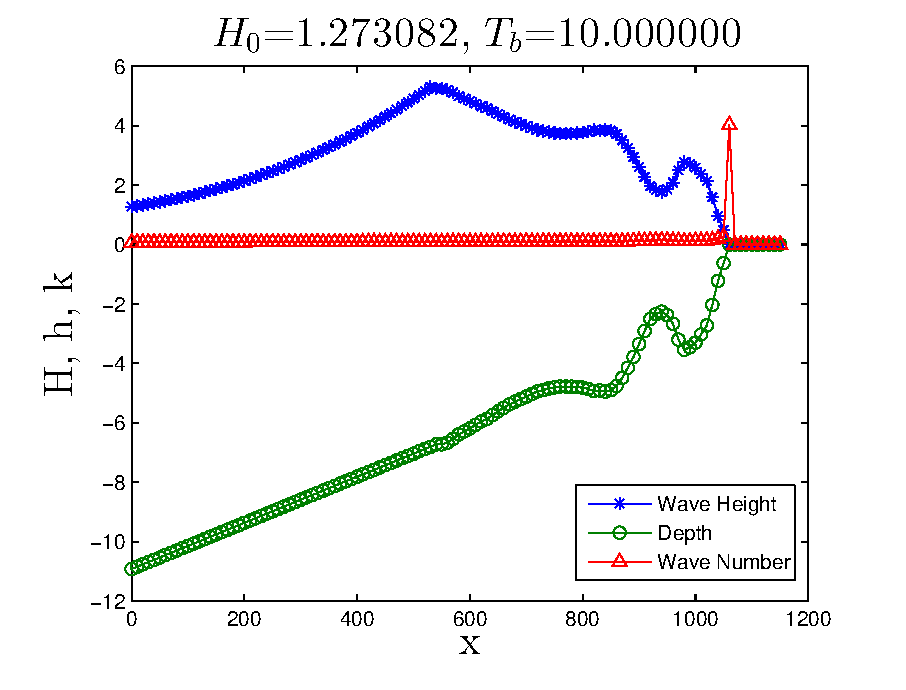
\includegraphics[width=\textwidth]{forward_plot/p1_1.eps}
%\caption{Case I: Water Depth(h), Wave Height(H) and Wave Number vary with x direction}
\label{FigHhk_1}
\end{minipage}
\hspace{0.2cm}
\begin{minipage}[b]{0.47\linewidth}
\centering
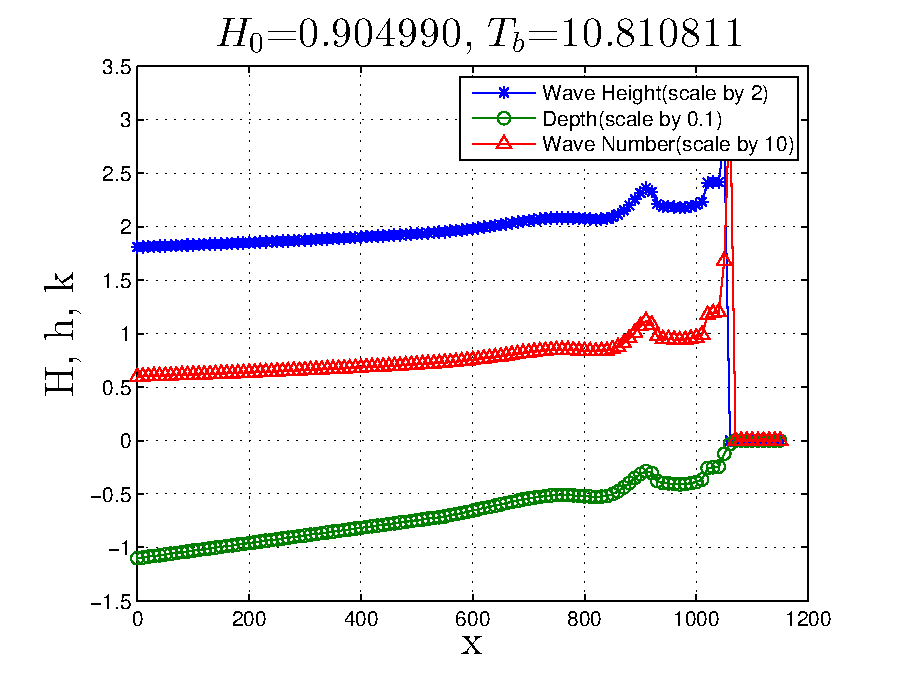
\includegraphics[width=\textwidth]{forward_plot/p2_1.eps}
%\caption{Case II: $N=500$}
\label{FigHhk_2}
\end{minipage}
\caption{Water Depth(h), Wave Height(H) and Wave Number vary along x direction (Two sets of boundary conditions are applied for following figures. The boundary conditions for the left is extracted from the data of 2015/10/9 22:00-23:00 and for the right is extracted from the data of 2015/10/9 03:00-04:00). Note that $x=0 m$ is located offshore at the boundary point.}
\end{figure}
%
Figure 2 shows that the wave height is positively correlated to the depth. We can see the similar characteristics between depth and wave number. This is the reason for why we can perform the simulation by providing ${H}$ or ${k}$ to obtain the depth ${h}$. The wave height curve and wave number curve will rapidly increase to a significant level around where depth is very close to zero, and the data there is not reliable because of the poor behavior of equations around $h=0 m$ (We need to force wave height to zero when depth is close to zero, or the wave height given by those equations will turn to infinity). However, the shape of wave height curve or wave number curve around the peak of depth curve shows our model has a reasonable good response to the changing depth.
Figure 3 shows the shallow water assumption which is $h*k<<1$ (The red horizontal line is $h*k=1$). We can see that our model is well fit the criteria at most data points except some where their depths are close to zero.
Figure 4 is the variation of wave energy along x-axis. The energy will accumulate unless the wave height meets the break condition.
Figure 5 is the variation of wave phase speed (celerity) along x-axis. As celerity is a function of wave number and wave period (wave period is assumed to be fixed in our case). 
Figure 6 shows the variation of wave height along with wave 
%%%%%%%%%%%%%%%%%%%%%%%%%%%%%%%%%%%%%%%%%%%%%%%%%%%%%%%%%%%%%%%%%%%%%%%%%%%%%%%%%%%%%%%%%%%%%%%%%%%%%%%%%%%%%%%%%%%%%%

%%%%%%%%%%%%%%%%%%%%%%%%%%%%%%%%%%%%%%%%%%%%%%%%%%%%%%%%%

\begin{figure}[h]
\begin{minipage}[b]{0.47\linewidth}
\centering
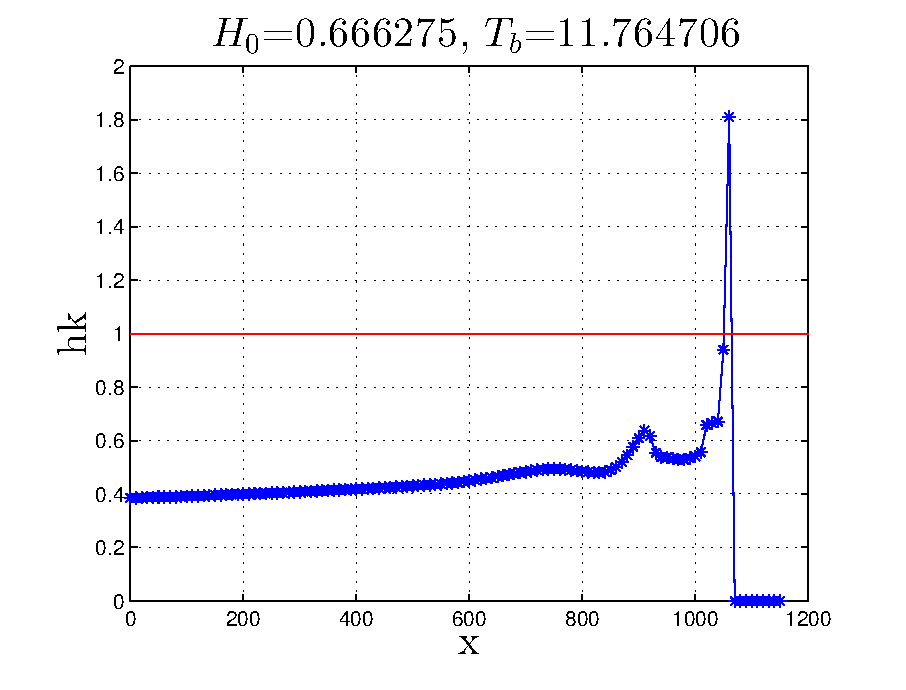
\includegraphics[width=\textwidth]{forward_plot/p1_2.eps}
%\caption{Example \eqref{ex1} Case I: $N=100$}
\label{Fighk_1}
\end{minipage}
\hspace{0.2cm}
\begin{minipage}[b]{0.47\linewidth}
\centering
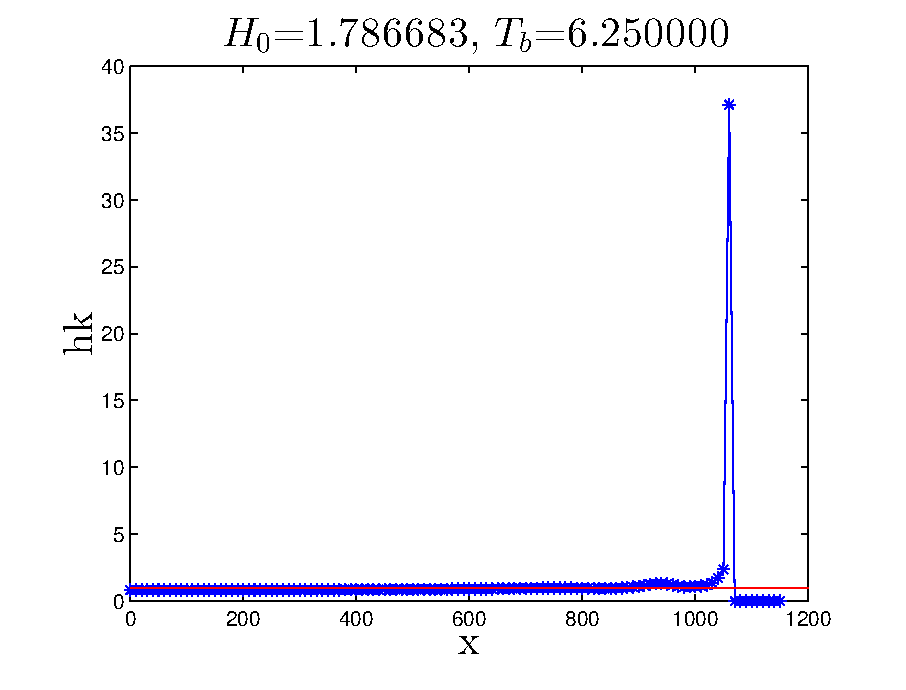
\includegraphics[width=\textwidth]{forward_plot/p2_2.eps}
%\caption{Example \eqref{ex1} Case I: $N=500$}
\label{Fighk_2}
\end{minipage}
\caption{Relative Depth varies with x direction}
\end{figure}
%%%%%%%%%%%%%%%%%%%%%%%%%%%%%%%%%%%%%%%%%%%%%%%%%%%%%%%%%%%%%%%%%%%%%%%%%%%%%%%%%%%%%%%%%%%%%%%%%%%%%%%%%%%%%%%%%%%%%%

%%%%%%%%%%%%%%%%%%%%%%%%%%%%%%%%%%%%%%%%%%%%%%%%%%%%%%%%%

\begin{figure}[h]
\begin{minipage}[b]{0.47\linewidth}
\centering
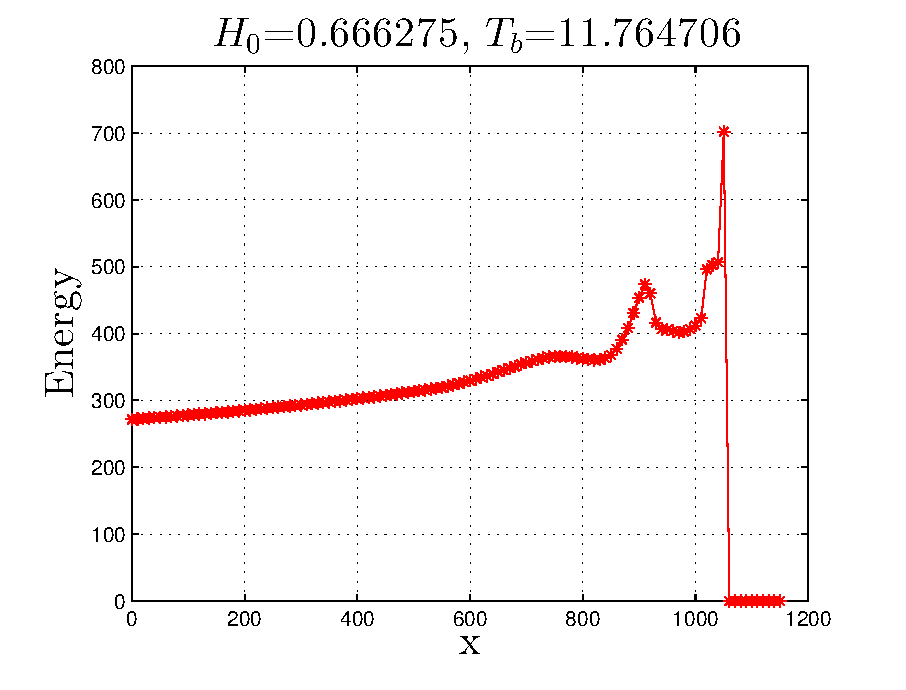
\includegraphics[width=\textwidth]{forward_plot/p1_3.eps}
%\caption{Example \eqref{ex1} Case I: $N=100$}
\label{Figenergy_1}
\end{minipage}
\hspace{0.2cm}
\begin{minipage}[b]{0.47\linewidth}
\centering
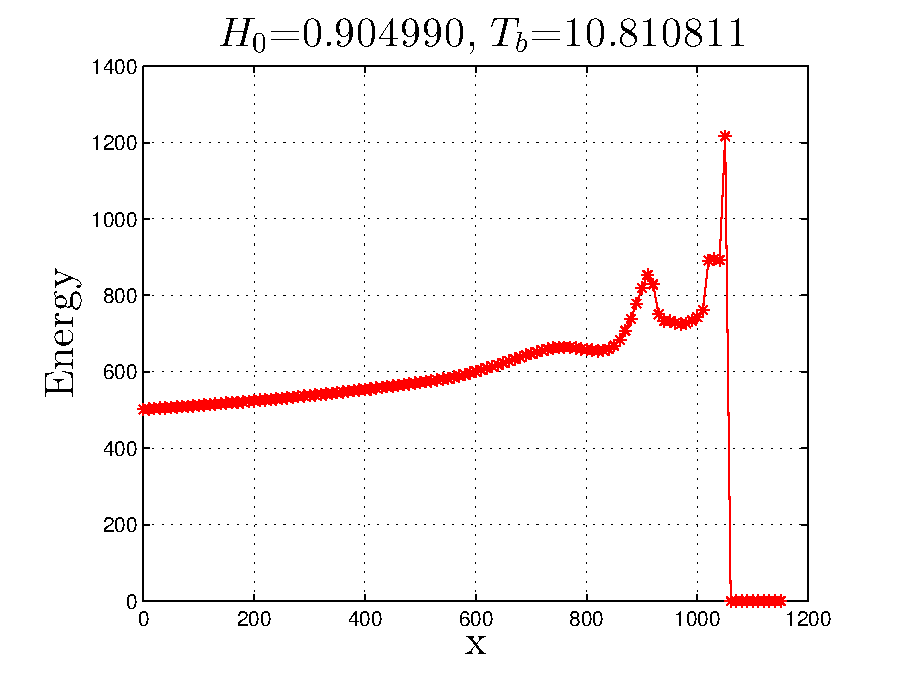
\includegraphics[width=\textwidth]{forward_plot/p2_3.eps}
%\caption{Example \eqref{ex1} Case I: $N=500$}
\label{Figenergy_2}
\end{minipage}
\caption{Wave Energy varies with x direction}
\end{figure}
%%%%%%%%%%%%%%%%%%%%%%%%%%%%%%%%%%%%%%%%%%%%%%%%%%%%%%%%%%%%%%%%%%%%%%%%%%%%%%%%%%%%%%%%%%%%%%%%%%%%%%%%%%%%%%%%%%%%%%

%%%%%%%%%%%%%%%%%%%%%%%%%%%%%%%%%%%%%%%%%%%%%%%%%%%%%%%%%

\begin{figure}[h]
\begin{minipage}[b]{0.47\linewidth}
\centering
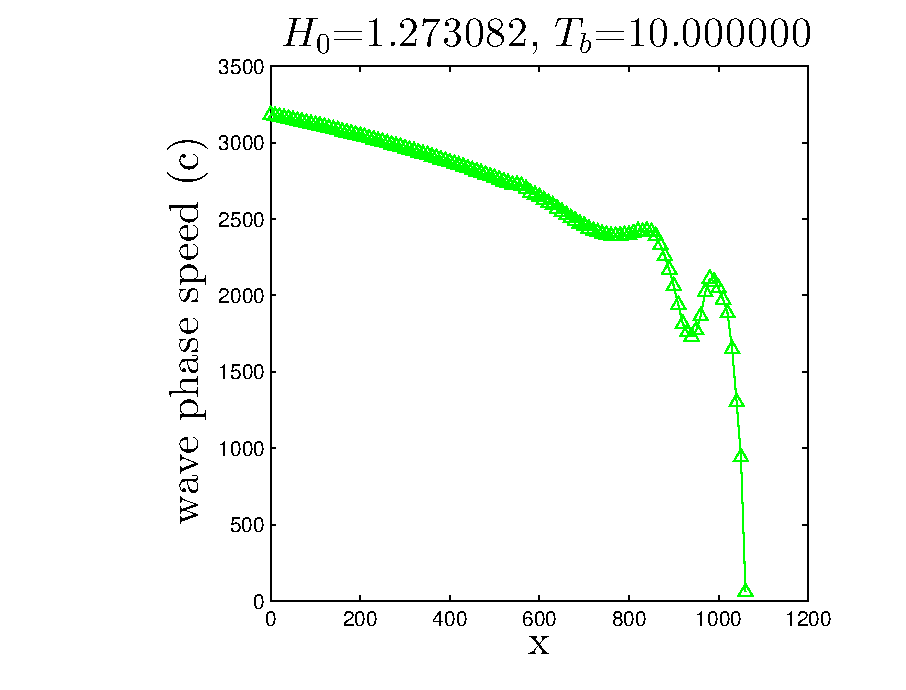
\includegraphics[width=\textwidth]{forward_plot/p1_4.eps}
%\caption{Example \eqref{ex1} Case I: $N=100$}
\label{Figc_1}
\end{minipage}
\hspace{0.2cm}
\begin{minipage}[b]{0.47\linewidth}
\centering
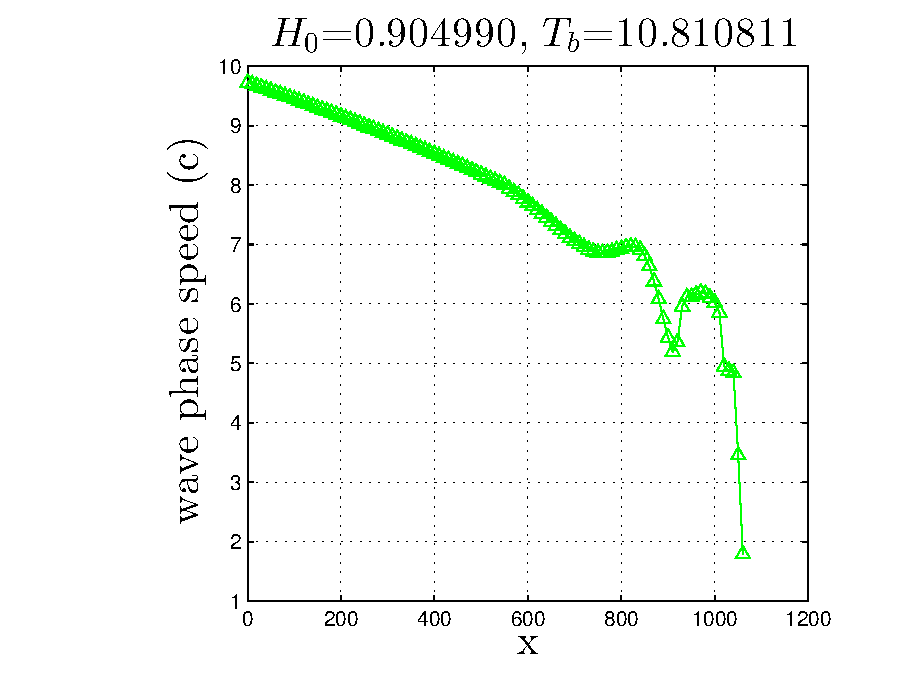
\includegraphics[width=\textwidth]{forward_plot/p2_4.eps}
%\caption{Example \eqref{ex1} Case I: $N=500$}
\label{Figc_2}
\end{minipage}
\caption{Wave Phase Speed (c) varies with x direction}
\end{figure}
%%%%%%%%%%%%%%%%%%%%%%%%%%%%%%%%%%%%%%%%%%%%%%%%%%%%%%%%%%%%%%%%%%%%%%%%%%%%%%%%%%%%%%%%%%%%%%%%%%%%%%%%%%%%%%%%%%%%%%%%%%%%%%%%%%%%%%%%%%%%%%%%%%%%%%%%%%%%%%%%%%%%%%%%%%%%%%%

\begin{figure}[h]
\begin{minipage}[b]{0.47\linewidth}
\centering
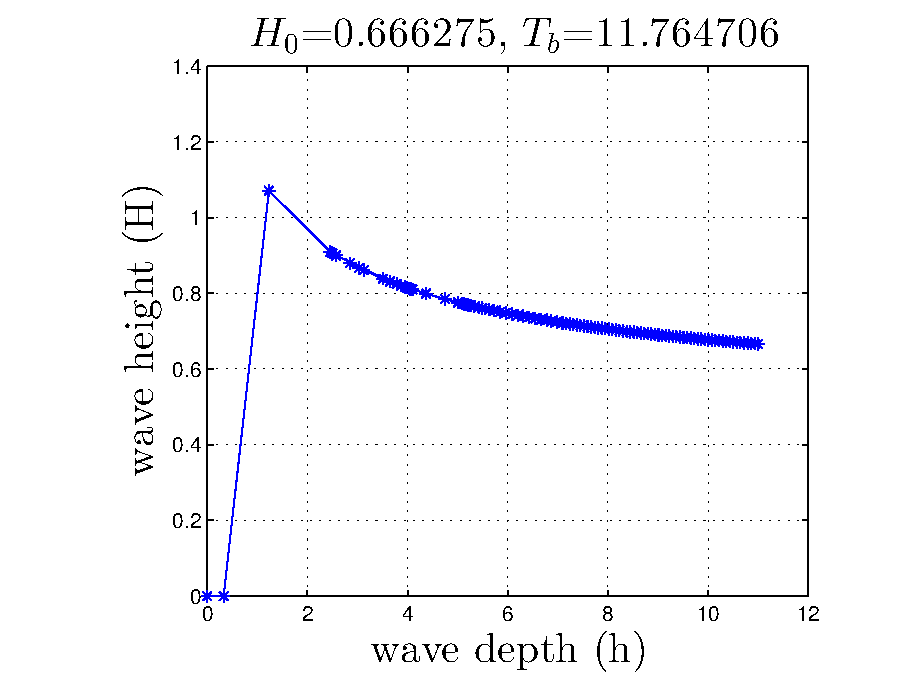
\includegraphics[width=\textwidth]{forward_plot/p1_5.eps}
%\caption{Example \eqref{ex1} Case I: $N=100$}
\label{FigH_1}
\end{minipage}
\hspace{0.2cm}
\begin{minipage}[b]{0.47\linewidth}
\centering
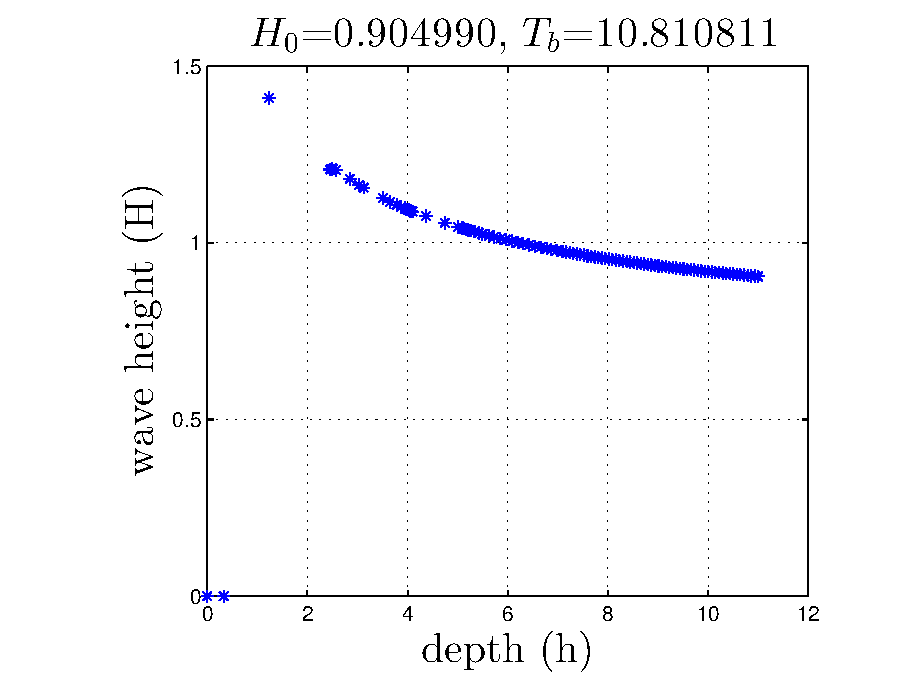
\includegraphics[width=\textwidth]{forward_plot/p2_5.eps}
%\caption{Example \eqref{ex1} Case I: $N=500$}
\label{FigH_2}
\end{minipage}
\caption{Wave Height(H) varies with Water Depth(h)}
\end{figure}
%%%%%%%%%%%%%%%%%%%%%%%%%%%%%%%%%%%%%%%%%%%%%%%%%%%%%%%%%%%%%%%%%%%%%%%%%%%%%%%%%%%%%%%%%%%%%%%%%%%%%%%%%%%%%%%%%%%%%%

%%%%%%%%%%%%%%%%%%%%%%%%%%%%%%%%%%%%%%%%%%%%%%%%%%%%%%%%%

\begin{figure}[h]
\begin{minipage}[b]{0.47\linewidth}
\centering
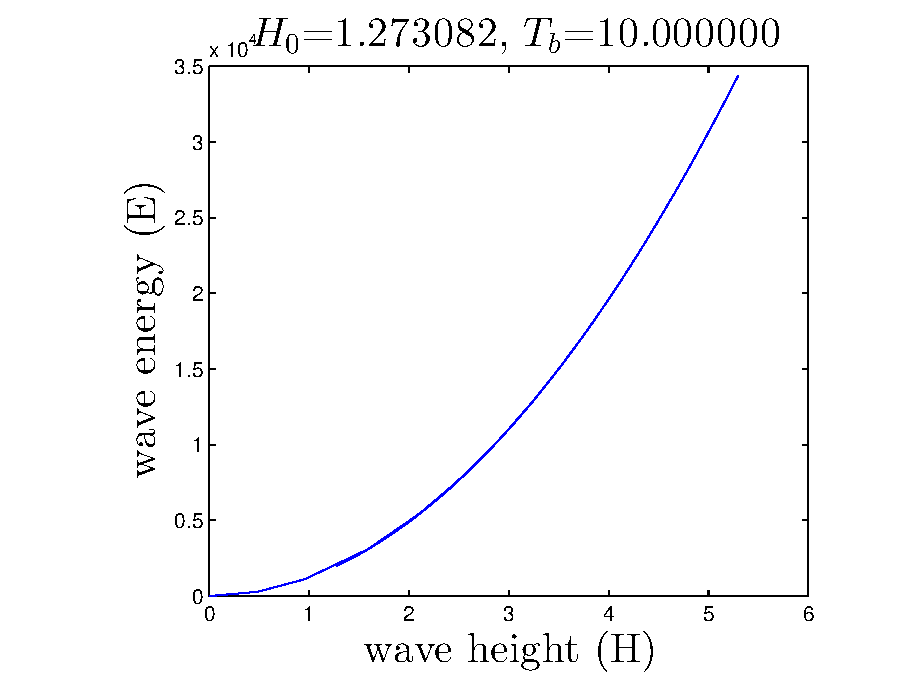
\includegraphics[width=\textwidth]{forward_plot/p1_6.eps}
%\caption{Example \eqref{ex1} Case I: $N=100$}
\label{FigE_1}
\end{minipage}
\hspace{0.4cm}
\begin{minipage}[b]{0.47\linewidth}
\centering
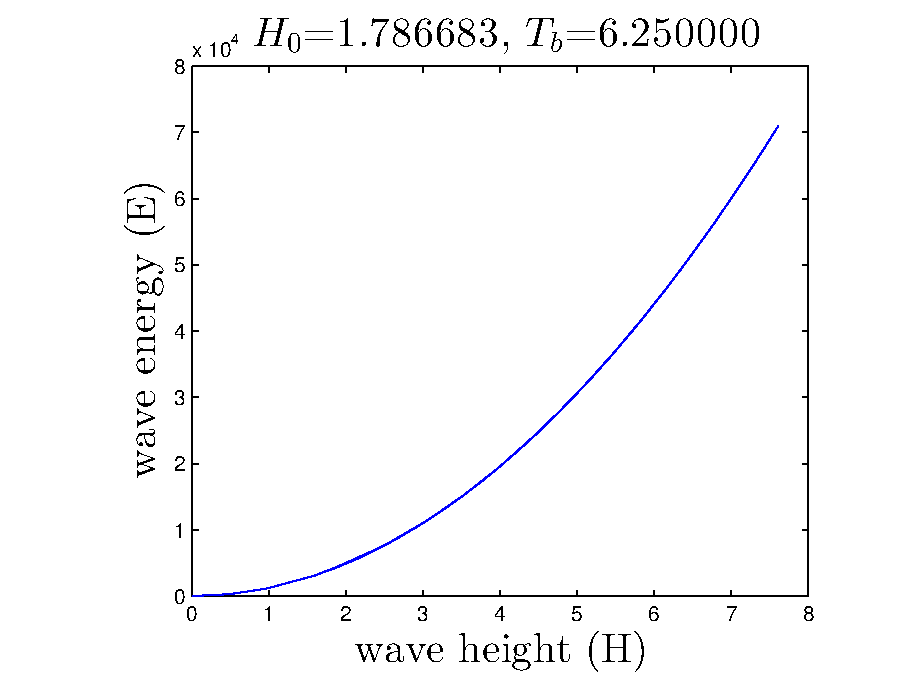
\includegraphics[width=\textwidth]{forward_plot/p2_6.eps}
%\caption{Example \eqref{ex1} Case I: $N=500$}
\label{FigE_2}
\end{minipage}
\caption{Wave Energy varies with Wave Height(H)}
\end{figure}
%%%%%%%%%%%%%%%%%%%%%%%%%%%%%%%%%%%%%%%%%%%%%%%%%%%%%%%%%%%%%%%%%%%%%%%%%%%%%%%%%%%%%%%%%%%%%%%%%%%%%%%%%%%%%%%%%%%%%%

\begin{figure}[h]
\begin{minipage}[b]{0.47\linewidth}
\centering
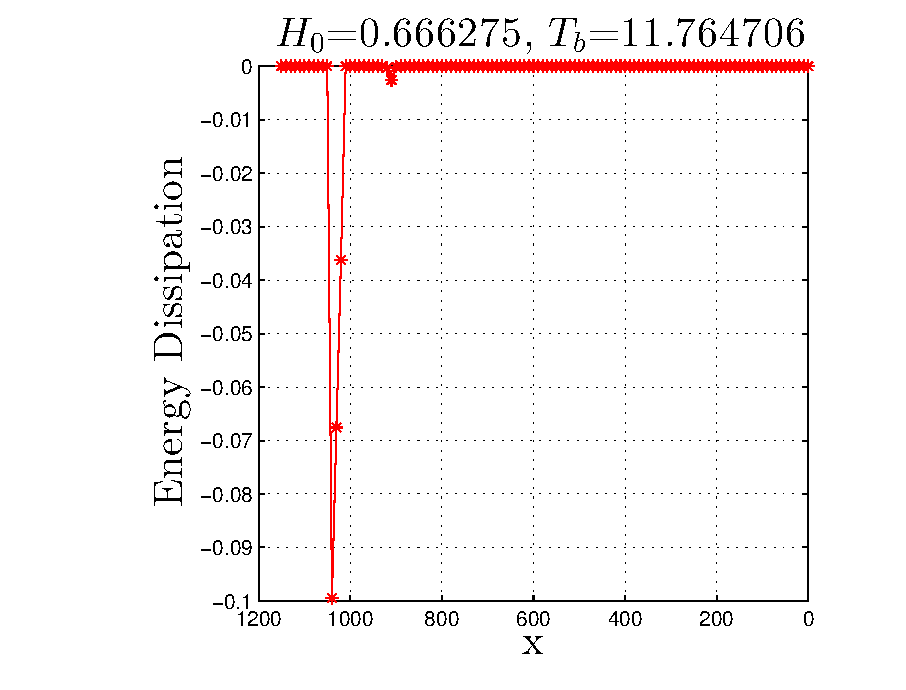
\includegraphics[width=\textwidth]{forward_plot/p1_7.eps}
%\caption{Example \eqref{ex1} Case I: $N=100$}
\label{FigE_1}
\end{minipage}
\hspace{0.4cm}
\begin{minipage}[b]{0.47\linewidth}
\centering
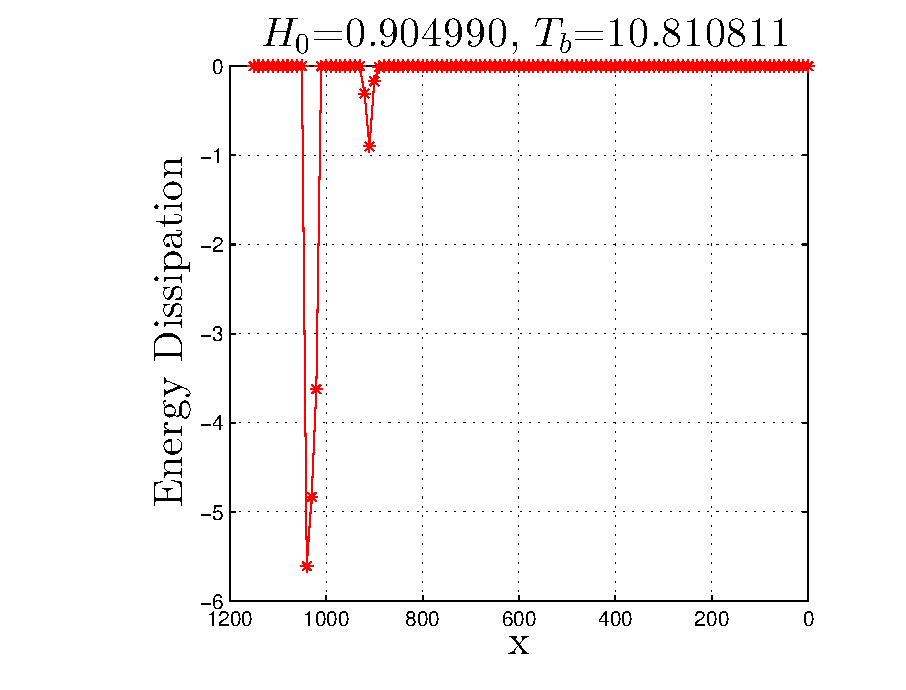
\includegraphics[width=\textwidth]{forward_plot/p2_7.eps}
%\caption{Example \eqref{ex1} Case I: $N=500$}
\label{FigE_2}
\end{minipage}
\caption{Wave Energy Dissipation varies along x-axis}
\end{figure}


\section{Data}
Data for this project were collected by the U.S. Army Corps of Engineers (USACE) Engineer Research and Development Center (ERDC) during October 2015 at the Field Research Facility (FRF) in Duck, NC on the Outerbanks shown in Figure~\ref{FRFmap}.\footnote{The data is available in netcdf format at http://chlthredds.erdc.dren.mil/thredds/catalog/frf/projects/bathyduck/catalog.html} The data was collected via the BathyDuck project conducted by the Coastal and Hydraulic Laboratory (CHL). Data of interest includes wave height (\textit{H}), wave number (\textit{k}), wave period (\textit{T}), and bathymetry (\textit{h}) measurements. These data combine information collected through a Nortek Acoustic Wave and Current (AWAC) Profiler, a Light Amphibious Resupply Cargo (LARC-5) vessel, a Coastal Research Amphibious Buggy (CRAB), and Argus Beach Monitoring systems. The LARC-5 and CRAB vessels are shown below in Figure ~\ref{crablarc}.

\begin{figure}[h]
\centering
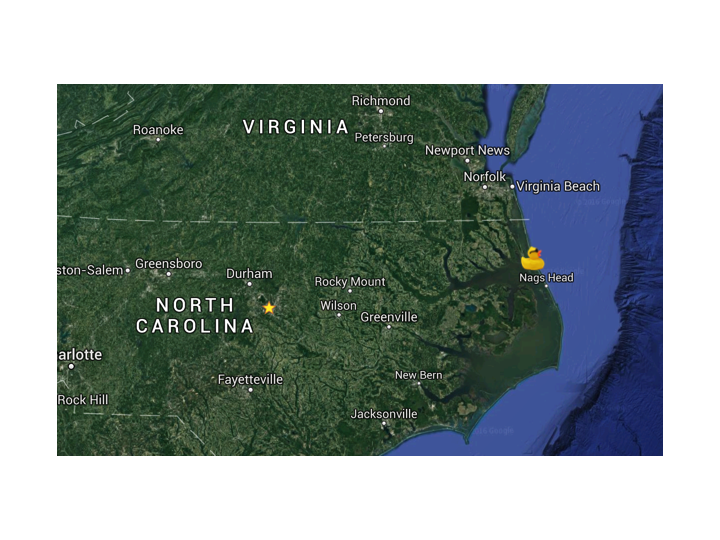
\includegraphics[width=7\linewidth]{img/FRF_map.png}
\caption{The location of the U.S. Army Corps of Engineers Field Research Facility in Duck, NC.}
\label{FRFmap}
\end{figure}

\begin{figure}[h]
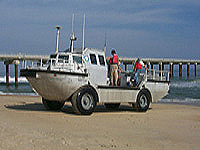
\includegraphics[width=.48\linewidth]{img/LARC.jpg}\hfill
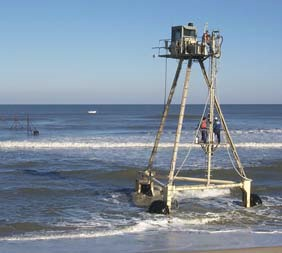
\includegraphics[width=.48\linewidth]{img/CRAB2.JPG}
\caption{The LARC (left) and CRAB (right) instruments are used to measure near coastal bathymetry. Image source: http://www.frf.usace.army.mil/aboutUS/equipment.shtml}
\label{crablarc}
\end{figure}

The following sections discuss in more detail the observations and how they were used. Note in physical space, the boundary point used for the 1-dimensional problem is located 1150 m offshore. For numerical simplicity, all observations are transformed such that $\textit{x}$ = 0 m corresponds to the offshore boundary point and $\textit{x}$ = 1150 m is the shoreline. 


\subsection{Boundary Condition}
\label{BC}

	Boundary conditions for this project were collected through a bottom-mounted AWAC profiler located approximately 1150 meters offshore at a depth of 11 meters (Figure \ref{AWAC}).

	\begin{figure}[h]
		\centering
		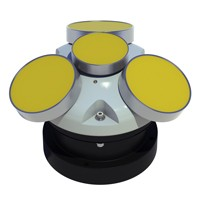
\includegraphics[width=.40\linewidth]{img/AWAC.jpg}
		\caption{Acoustic Wave and Current Profiler. Image source: http://www.nortek-as.com/en/products/wave-systems/awac}
		\label{AWAC}
	\end{figure}
	
	Vast amounts of wave data has been collected by the AWAC system at the offshore boundary. For the 1-dimensional problem, the forcing condition at this boundary is the significant wave height and peak frequency.
\subsection{Bathymetry}
\label{sec: bathy}

	Survey data collected on 1 October 2015 was considered for this analysis. These data were measured via the CRAB and Trimble Real Time Kinematic (RTK) GPS system. Elevation data from six cross-sections\footnote{we could potentially add an overhead plot of the transects}, perpendicular to the shoreline, spaced over a 100-meter portion of the beach were combined to create the 2D surface shown in Figure \ref{2D Bath}. 
	
	 	\begin{figure}[H]
	 	\centering
	 	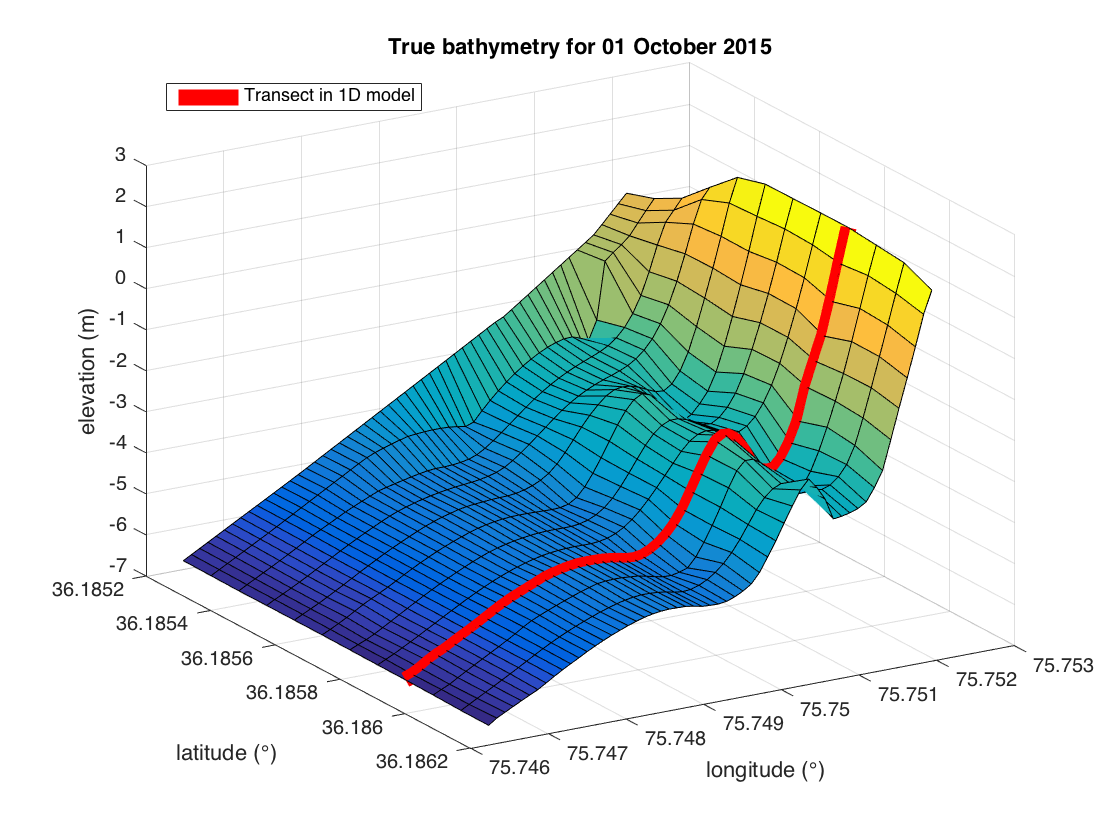
\includegraphics[width=0.6\linewidth]{img/trueBath2D.png}
	 	\caption{Measured and gridded 2D bathymetry in the survey area on 1 October 2015. The red line shows the transect considered in the 1D problem.}
	 	\label{2D Bath}
	 	\end{figure}
	
	For the 1D problem, a single slice of the 2D bathymetry was used as model input, identified by the red line in Figure \ref{2D Bath}. In a cartesian coordinate system, this line (a.k.a. `transect') is located at \textit{y} = 950 meters. 
		
		\begin{figure}[H]
		\centering
		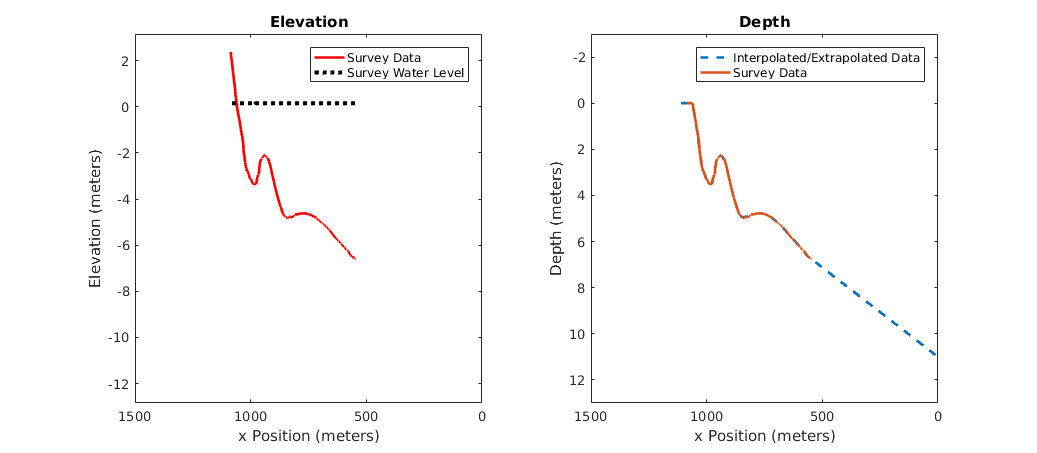
\includegraphics[width = 1.0\linewidth]{img/trueBath1D.png}
		\caption{1D Bathymetry - elevation data (left) and depth data (right).}
		\label{1D Bath}
		\end{figure}
		
	Survey data provided sea floor elevation referenced to the North American Vertical Datum of 1988 (NAVD88) (Figure \ref{1D Bath}, \textit{left}). To provide proper input data for the 1D model, elevation was transformed to depth data (Figure \ref{1D Bath}, \textit{right}). Once transformed, depth was discretized by interpolating between measured data points via Matlab's built-in pchip method. Pchip was chosen for the interpolation due to its shape-preserving nature so as to not introduce non-physical oscillations. Between the boundary condition and the nearest measured depth point, linear interpolation was used to fill in missing data.
\subsection{Wave number}

Wave number is a measure of the number of waves per unit distance and is inversely proportional to wave speed. Hourly observations  using an Argus video monitoring system mounted on shore are available during October 2015. Photogrammetry is performed on the video to derive the dominant wave frequencies and wave numbers in the survey area \citep{holman2013}. Data is available for a 2D area at the FRF survey site. A 1D profile is extracted from the 2D data along a transect corresponding to the position of the model boundary point (\textit{y} = 950 m). Figure~\ref{k1Dmean} shows statistics for wave number, \textit{k}, along the 1D transect. Wave number is shown to be more variable over time further from the coastline. Mean wave number decreases toward the shoreline, as expected.



\begin{figure}[h]
\centering
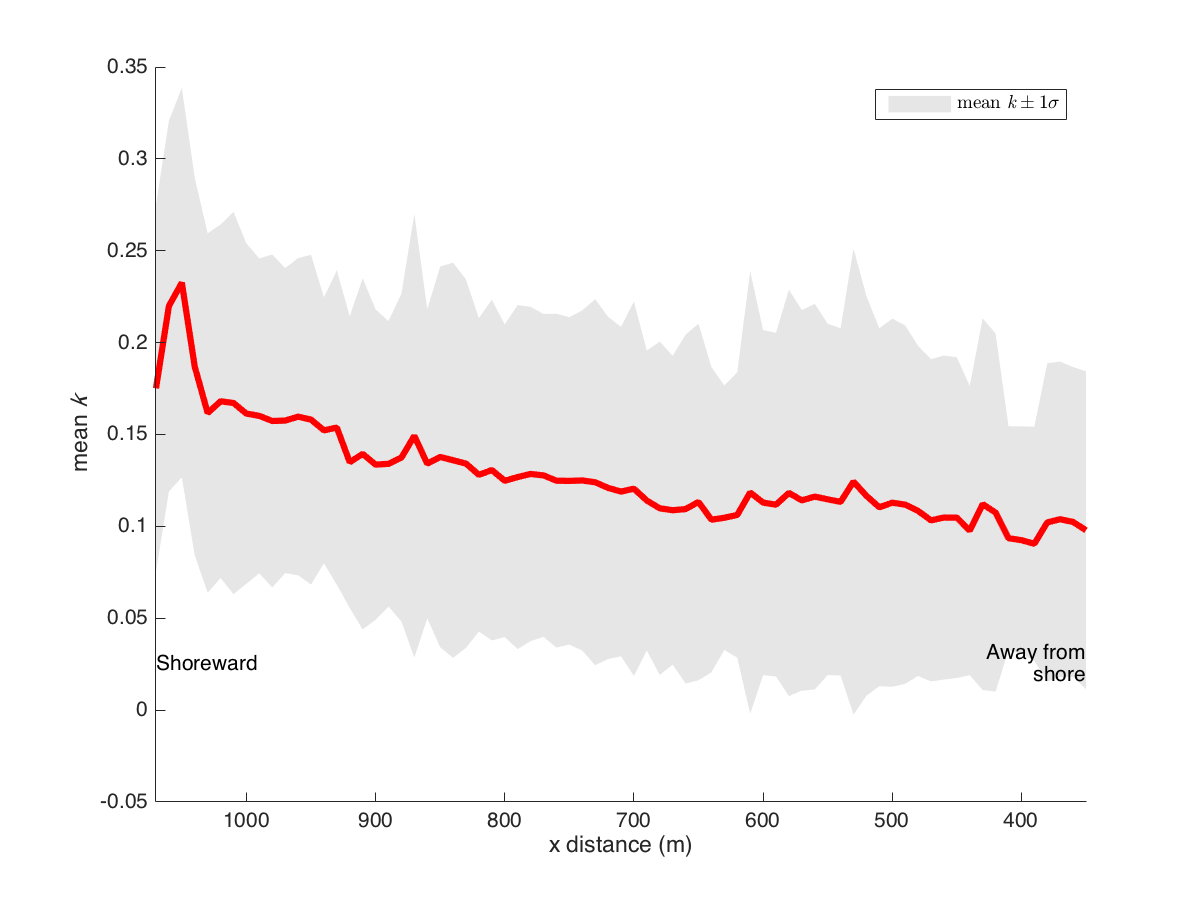
\includegraphics[width=.55\linewidth]{img/k1Dmean_std.png}
\caption{Wave number along the transect where the model boundary condition is located. Mean wave number, \textit{k}, during October 2015 is shown in red. Gray envelopes show $\pm$ 1$\sigma$ standard deviation in \textit{k}. Wave number is observed to be relatively larger and more variable further from shore.}
\label{k1Dmean}
\end{figure}

\section{The Approach}

In this section, we are going to perform a preliminary study about potential inversion schemes that we can use to recover the unknown bathymetry parameter with the given measurements and the given forward model. In particular, we test and validate six different inversion methods with artifically generated dataset by assuming those data is corrupted by Gaussian noise. 

\subsection{The Additive Gaussian Noise Model} \label{Gaussian_noise}
By assuming the measurements are corrupted by the additive Gaussian noise, the linear estimation model can be written as 
\begin{equation}
\mathbf{d} \sim \text{Gaussian}( \mathbf{A} \mathbf{h}_t),
\end{equation}
\vspace{0.3cm}
where\\
\begin{tabular}{l c l}
$\mathbf{d}$ &=& a vector of measurements,\\
$\mathbf{A}$ &=& a linear forward operator,\\
$\mathbf{h}_t$ &=& the true bathymetry (depth). 
\end{tabular}

\vspace{0.3cm}
\noindent Therefore, a Gaussian noise $\boldsymbol{\epsilon}$ corrupted measurements $\mathbf{d}$ with a standard deviation  $\nu$ is given by 
$$
\mathbf{d} = \mathbf{A} \mathbf{h}_t + \boldsymbol{\epsilon}.
$$



\subsection{Ordinary Least-Squares Inversion}

%\subsubsection{Least-Squares Inversion}

As a beginning to approximate the topographic heights of the near-shore sea-floor,  we consider the following least-squares minimization problem,
\begin{equation}\label{LS}
\mathbf{\hat{h}}= \underset{\mathbf{h} \in \mathbb{R}^n}{\arg \min} \ \ f(\mathbf{h}) = \|  \mathbf{A}\mathbf{h} -  \mathbf{d} \|_2^2,
\end{equation}
where we minimize the data misfit between the forward predictions and the measurements, in the least-squares sense. In order to test possible Matlab\textsuperscript{\textregistered} inbuilt solvers to solve the minimization problem in  \eqref{LS}, we have generated dummy measurements with $\nu = 0.1$. In particular, in this test, the forward operator \verb|A = rand(50)|, the true bathymetry \verb| ht = -linspace(-11,0,N)'| \verb|- 11|, and the Gaussian noise corrupted measurements \verb|b = A * h_t + 0.1 * randn(N,1)|. Recovered bathymetries from different Matlab\textsuperscript{\textregistered} solvers are given below. Note that the initial guess for all methods is zero. 
\begin{itemize}
\item[(1)]  \textit{Nonnegative least-squares method:}  \verb|lsqnonneg(A,b, options)|. This Matlab\textsuperscript{\textregistered} function uses the algorithm so called \textit{active-set} and note that it requires the matrix $\mathbf{A}$ explicitly. Residual norm error for this nonnegativity reconstruction is $8.88 \times 10^{-26}$ (see Fig. \ref{nonLS_fig}).   \\

\begin{figure}[H]
\center
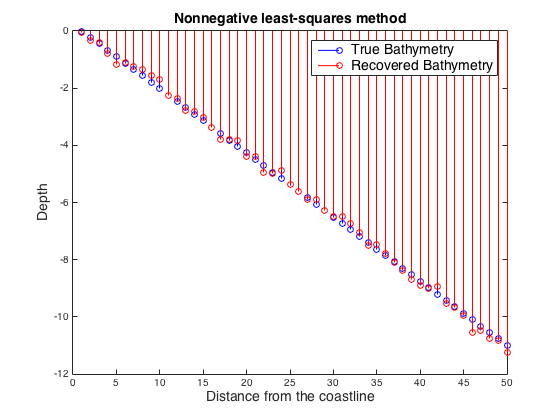
\includegraphics[scale=0.6]{img/NonLS_linear.png} 
\caption{Nonnegative least-squares method reconstruction of depth $\mathbf{h}$ using the dummy dataset.}
\label{nonLS_fig}
\end{figure}
\item[(2)]  \textit{Trust-Region-Reflective method:}  \verb|lsqnonlin(@(h) A * h - b, zeros(N,1),| \\ \verb|zeros(N,1),inf(N,1), options)|. Note that the reconstruction of $\mathbf{h}$ is restricted to the positive x-axis using the function arguments. Residual norm error for the reconstruction is $4.32 \times 10^{-10}$. 
\begin{figure}[H]
\center
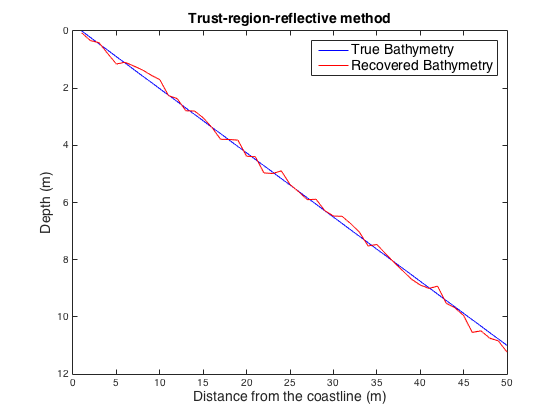
\includegraphics[scale=0.6]{img/trust_region_linear.png} 
\caption{Trust-Region-Reflective method reconstruction of depth $\mathbf{h}$ using the dummy data.}
\label{trust_region_fig}
\end{figure}
\item[(3)]  \textit{Levenberg-Marquardt (LM) method:}  
\verb|lsqnonlin(@(h) A * h - b, 'Algorithm',| \\ \verb|'levenberg-marquardt')|
Residual norm error for the reconstruction is $6.39 \times 10^{-13}$. The Levenberg-Marquardt algorithm does not handle bound constraints. 
\begin{figure}[H]
\center
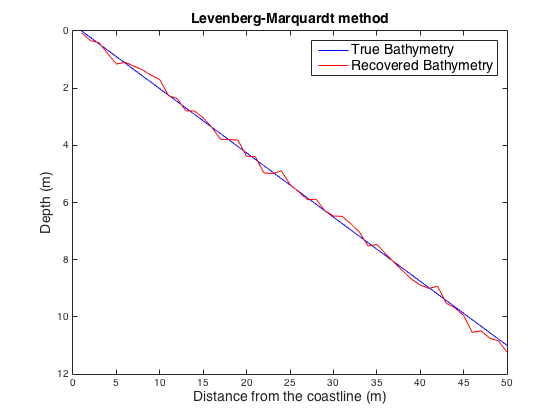
\includegraphics[scale=0.6]{img/LM_linear.png} 
\caption{Levenberg-Marquardt (LM) method reconstruction of depth $\mathbf{h}$ using the dummy data.}
\label{LM_fig}
\end{figure}
\item[(4)]  \textit{Interior-point method:} \verb|fmincon(f, zeros(N,1), [],[],[],[], zeros(N,1), inf(N,1))|. Residual norm error for the sample dummy data set  with $\nu = 0.1$ is $1.29$. 
\begin{figure}[H]
\center
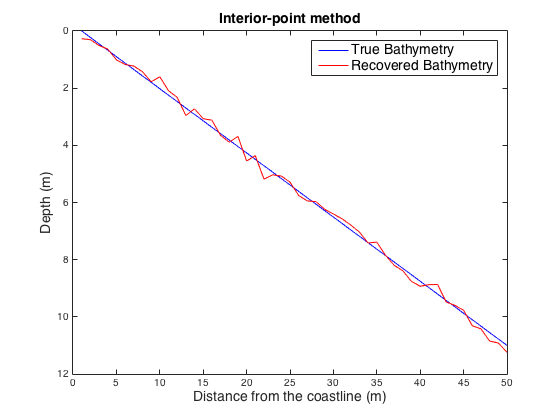
\includegraphics[scale=0.6]{img/fmincon_linear.png} 
\caption{fmincon method reconstruction of depth $\mathbf{h}$ using the dummy data.}
\label{LM_fig}
\end{figure}
\end{itemize}



\subsection{ Tikhonov Regularization}\label{TikRegMethod}

Although the ordinary least squares solution can deal with well-posed problems (i.e. the solution exist and unique), it might yield into a unstable solutions in the presence of a small noise in the measurements. Due to the ill-conditioned nature of the forward operator matrix $\mathbf{A}$, the noise components of the observations can be amplified and leads into a drastic change in the solution \cite{Tuys2014}. To overcome this problem, we use \textit{regularization}. The Tikhonov regularization is one of the most widely used regularization techniques in the inverse problems community. It couples the least squares term in \eqref{LS} with a additional regularization term as defined by 
\begin{equation}\label{eq:TR}
\mathbf{\hat{h}} = \underset{\mathbf{h} \in \mathbb{R}^n}{\arg \min} \ \ \|  \mathbf{A}\mathbf{h} -  \mathbf{d} \|_2^2  +  \alpha \| \mathbf{h}\|_2^2
\end{equation}
where $\alpha$ is the regularization parameter ($>0$), which balances the trade-off between data fidelity term (i.e, the least squares term) and the regularization term $\| \mathbf{h}\|_2^2$. %In particular, while the generalized solution strives to fit to the data, the noise components of the observations can be amplified by the forward operator. This leads into so the solution may drastically change. This behavior is due to the ill-conditioned nature of the forward operator matrix $\mathbf{A}$. 
Last but not least, the ordinary least squares method can not incorporate any prior knowledge about the bathymetry, for e.g., any known depths near the shore. However, If we have  some prior depth estimate $\mathbf{h}_p$ for the $\mathbf{h}_t$, then the Tikhonov regularized solution with the prior information can be written as
\begin{equation}\label{eq:TR-prior}
\mathbf{\hat{h}} = \underset{\mathbf{h} \in \mathbb{R}^n}{\arg \min} \  \|  \mathbf{A}\mathbf{h} -  \mathbf{d} \|_2^2  +  \alpha \| \mathbf{h} -  \mathbf{h}_p\|_2^2,
\end{equation}
where $\alpha$ is a regularization parameter $(>0)$. To test this method in \eqref{eq:TR-prior}, Tikhonov method is implemented and tested with sample data set with $\nu = 0.2$. This reconstruction of depth has 0.038 residual norm error. Note that the \verb|tikhonov| Matlab\textsuperscript{\textregistered} function requires the matrix $\mathbf{A}$ explicitly in order to solve the Tikhonov regularized minimization problem. 

\begin{figure}[H]
\center
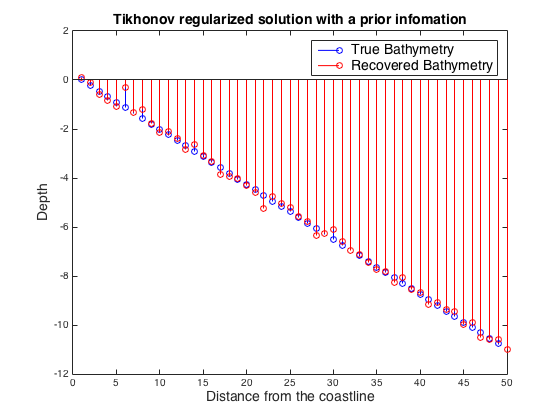
\includegraphics[scale=0.6]{img/Tikhnove_reg.png} 
\caption{The \textit{tikhonov }Matlab\textsuperscript{\textregistered} function reconstruction of the depth using the dummy data.}
\label{TR-recon}
\end{figure}

%In order to use the \verb|tikhonov| Matlab function to solve \eqref{eq:TR} or \eqref{eq:TR-prior}, the matrix $\mathbf{A}$ in should be explicitly known as a matrix. However, according to the our model derivation, forward model is nonlinear and it can not be wrtting  Therefore, we have to use some general Matlab 

%Reference: I found a MATLAB package for analysis and solution of discrete ill-posed problems, which is available in http://www2.imm.dtu.dk/~pcha/Regutools/\\








%\subsection{Help}
%
%LSQR method: $\hat{\Psi}$ = lsqr(A,d,tol,maxit) it attempts to solve the least squares solution x that minimizes norm$(\mathbf{d}-\mathbf{A\Psi})$ Note that $\mathbf{A}$ need not be square.
%
%
%Conjugate gradients: $\hat{\Psi}$ = cgs(A,b) attempts to solve the system of linear equations $\mathbf{A}\mathbf{\Psi} -  \mathbf{d}$ for $\Psi$.
%
%
%why fmincon: \url{http://www.mathworks.com/help/optim/ug/choosing-a-solver.html#bsbwxm7}


\subsection{Bayesian MCMC Inverse Method}

The Bayesian MCMC Method can be used with the Forward Model to gather an estimate for depth, \textit{h}, given wave number, \textit{k}, and wave height, \textit{H}. To estimate depth, we had to create a prior distribution function of bathymetry with given samples of depths from (add location).  Given the sample bathymetry, we inputed these values in the Forward Model to produce wavelengths and wave numbers. This model is then compared with a function of parameters \textit{k} and \textit{H} given depth, formally known as a likelihood function to compare the simulated data with the survey data from (location). This makes a good estimate of the depths to create a distribution of depths profile, known as the posterior probability function.  The modeled relationship is given by equation below


$$P(h|H,k) \propto P(h)L(h|H,k),$$ 

$$P(h)=$$

\[ L(h|H,k)=\sum\limits_{i=1}^n \frac{(\bar{k}-k_{i})^2}{\sigma_{i}^2}\]


and $P(h|H,k)$ represents the posterior probability function, $P(h)$ is the prior distribution function and $L(h|H,k)$ is the likelihood function.

%\begin{equation}
%\end{equation}






%\subsection{Estimating Bathymetry}

In this Section, we describe some experimental results with simulated and real data using few existing nonlinear optimization tools that we used in our preliminarily experiments (see Section \ref{inv_techniques}). Note that our forward model is nonlinear as described in Section \ref{forwardproblem} and it can not be written as a matrix equation system. Therefore, in this Bathymetry inversion, we can not use any inverting method where it needs forward operator as a explicit matrix operator (e.g., \verb|tikhonov| and  \verb|lsqnonneg|     
 Matlab\textsuperscript{\textregistered} functions need forward operator as a matrix). Moreover, the bounds of the true Bathymetry range in the interested near shore region is known to be $[0m, 11m]$. Therefore, we picked the inverse solvers that enables us to incorporate that prior knowledge too. 

\subsection{Simulated Data}
In this study, Gaussian noise corrupted simulated wave numbers (see Section \ref{Gaussian_noise} for more details) are generated by 
\begin{equation}
\mathbf{k}_s = A(\mathbf{h}_t) + \mathcal{N}(0, \nu^2),
\end{equation}
where $A(\cdot)$ represents the nonlinear forward operator defined in Section \ref{forwardproblem}, $\mathbf{h}_t \in \mathbb{R}_+^n$ is the true Bathymetry vector, and $\mathcal{N}(0, \nu^2)$ is a additive Gaussian noise vector with standard deviation $\nu$, generated in the Matlab\textsuperscript{\textregistered} by $\nu \cdot $\verb| randn(n,1)|. we manufactured wave numbers $\mathbf{k}_s$ for two different grid resolutions, i.e., 10m and 25m (see Fig. \ref{Simulated10m} and \ref{Simulated25m} respectively), to test and tune our inverse methods before working with actual measurements. 



\begin{figure}[H]
\center
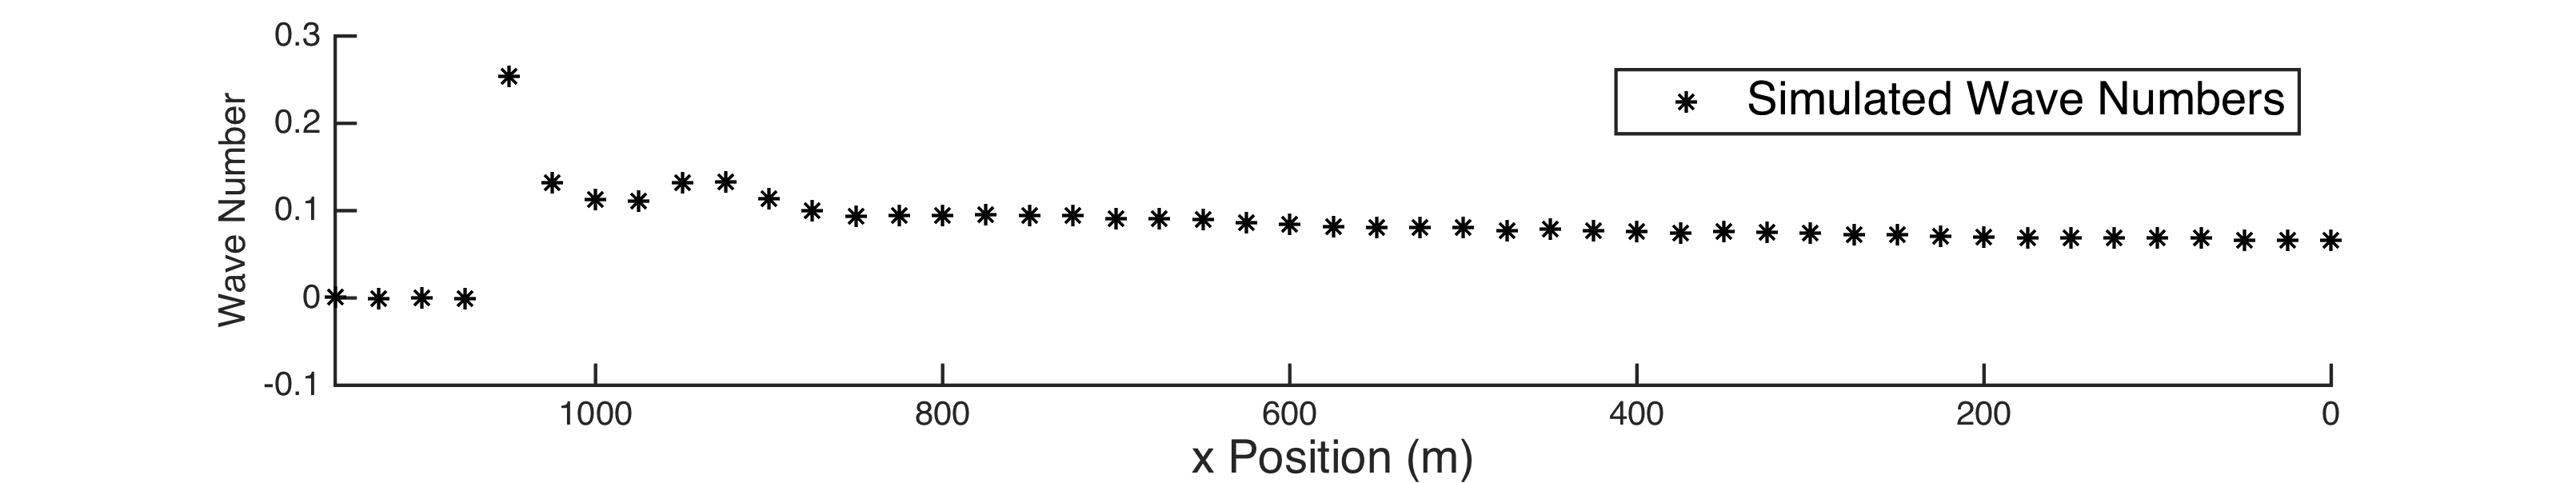
\includegraphics[scale=0.6]{img/simulated_data_k25m.png} 
\caption{1\% noisy ($\nu = 10^{-3}$) simulated wave numbers $(k)$ with 25m grid resolution. Noise (\%) = $\|A(\mathbf{h}_t) -  \mathbf{k}_s\| / \|  \mathbf{k}_s \| \cdot 100$.}
\label{Simulated25m}
\end{figure}

\begin{figure}[H]
\center
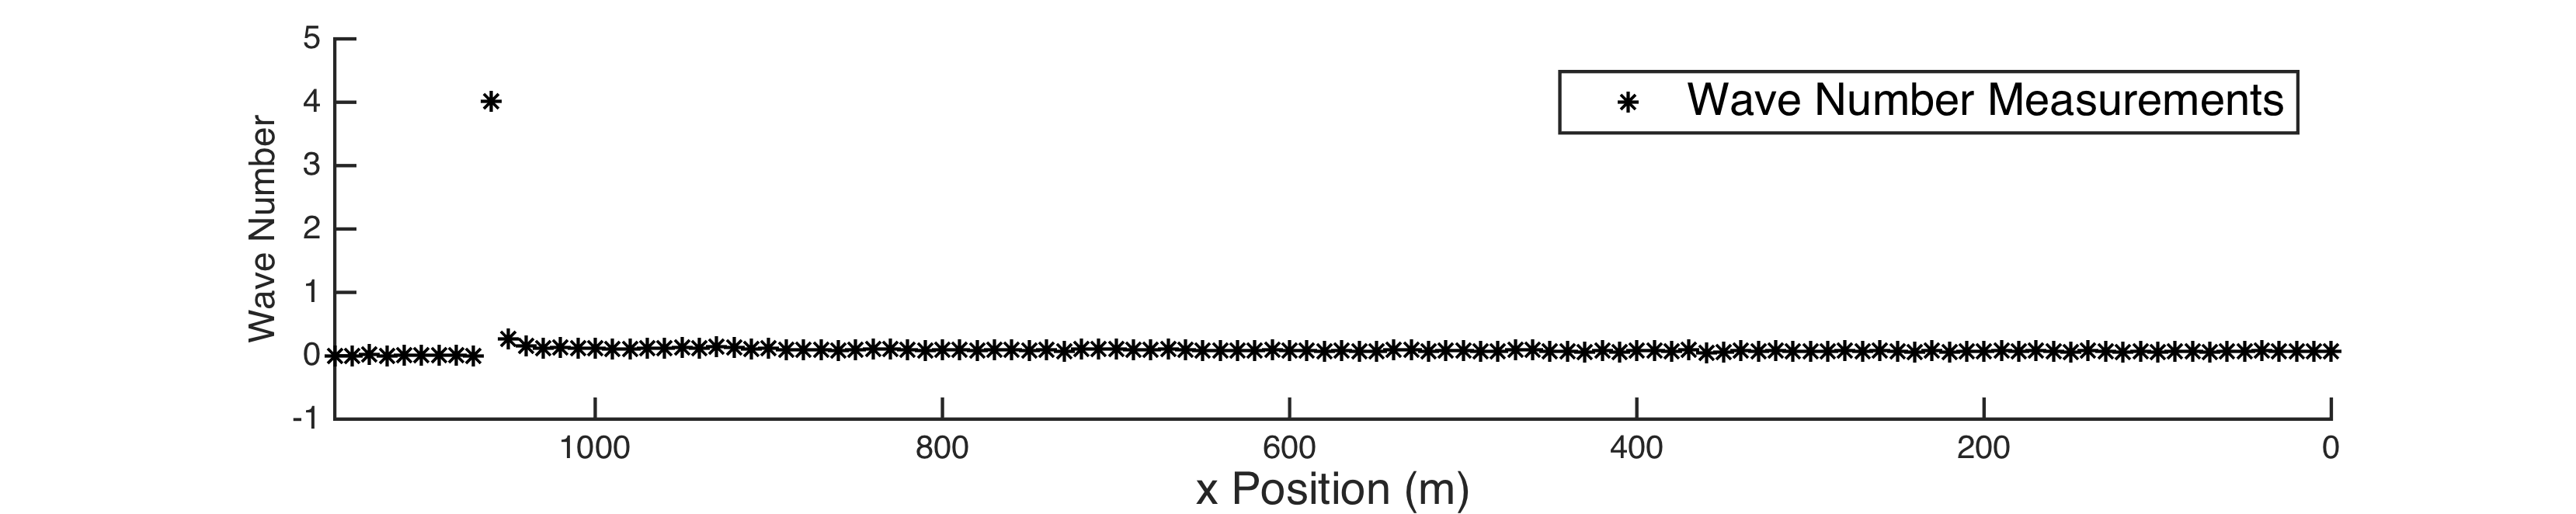
\includegraphics[scale=0.6]{img/simulated_data_k10m.png} 
\caption{2.5\% ($\nu = 10^{-2}$) noisy simulated wave numbers $(k)$ with 10m grid resolution. Noise (\%) = $\|A(\mathbf{h}_t) -  \mathbf{k}_s\| / \|  \mathbf{k}_s \| \cdot 100$. }
\label{Simulated10m}
\end{figure}


\subsection{Real Data}


Measured wave numbers (see Fig. \ref{RealData_oct09}) by US Army Corps of Engineers (USACE) at the field research facilities in Duck, NC on 09th October 2015  is used to approximate the true bathymetry using different inversion schemes. Note that the measured wave numbers near the shore (x Position $>$ 1050m) and the deep end (x Position $<$ 350m) are not available for our numerical experiments. 

\begin{figure}[H]
\center
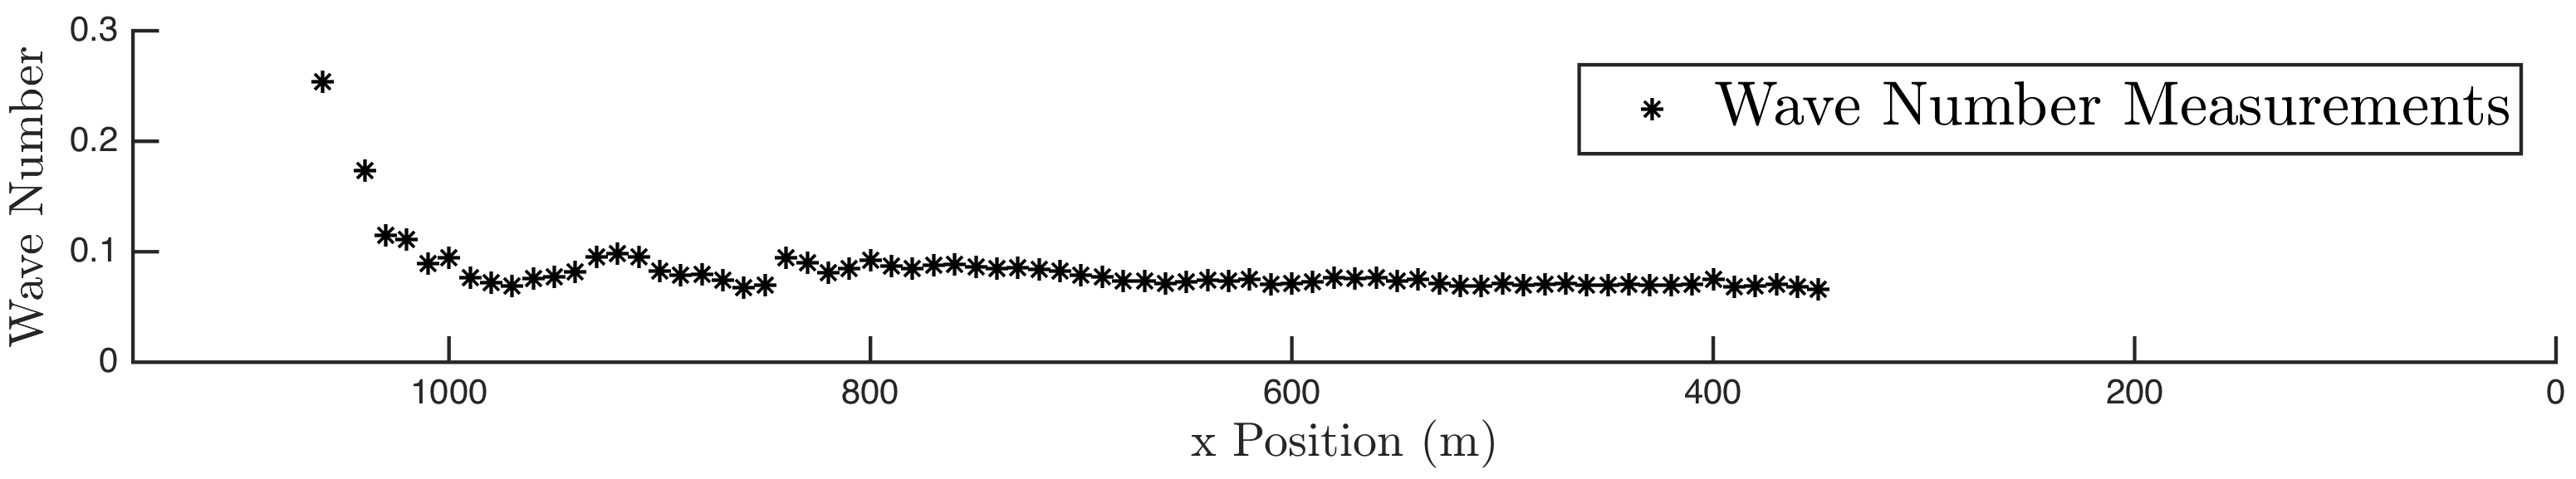
\includegraphics[scale=0.5]{img/real_data_k_Oct09.png} 
\caption{Real measurements of wave numbers $(k)$ on the 09th October 2015 at 21:59 by the US. Army Corps of Engineers (USACE) Engineer Research and Development Center (ERDC).}
\label{RealData_oct09}
\end{figure}




\subsection{Ordinary Least-Squares Fitting}


\begin{equation}\label{LS-BC}
\mathbf{\hat{h}}= \underset{\mathbf{0} \preceq \mathbf{h} \preceq \mathbf{11} }{\arg \min} \ \  \|  \mathbf{A}(\mathbf{h}) -  \mathbf{d} \|_2^2,
\end{equation}

\begin{figure}[H]
\center
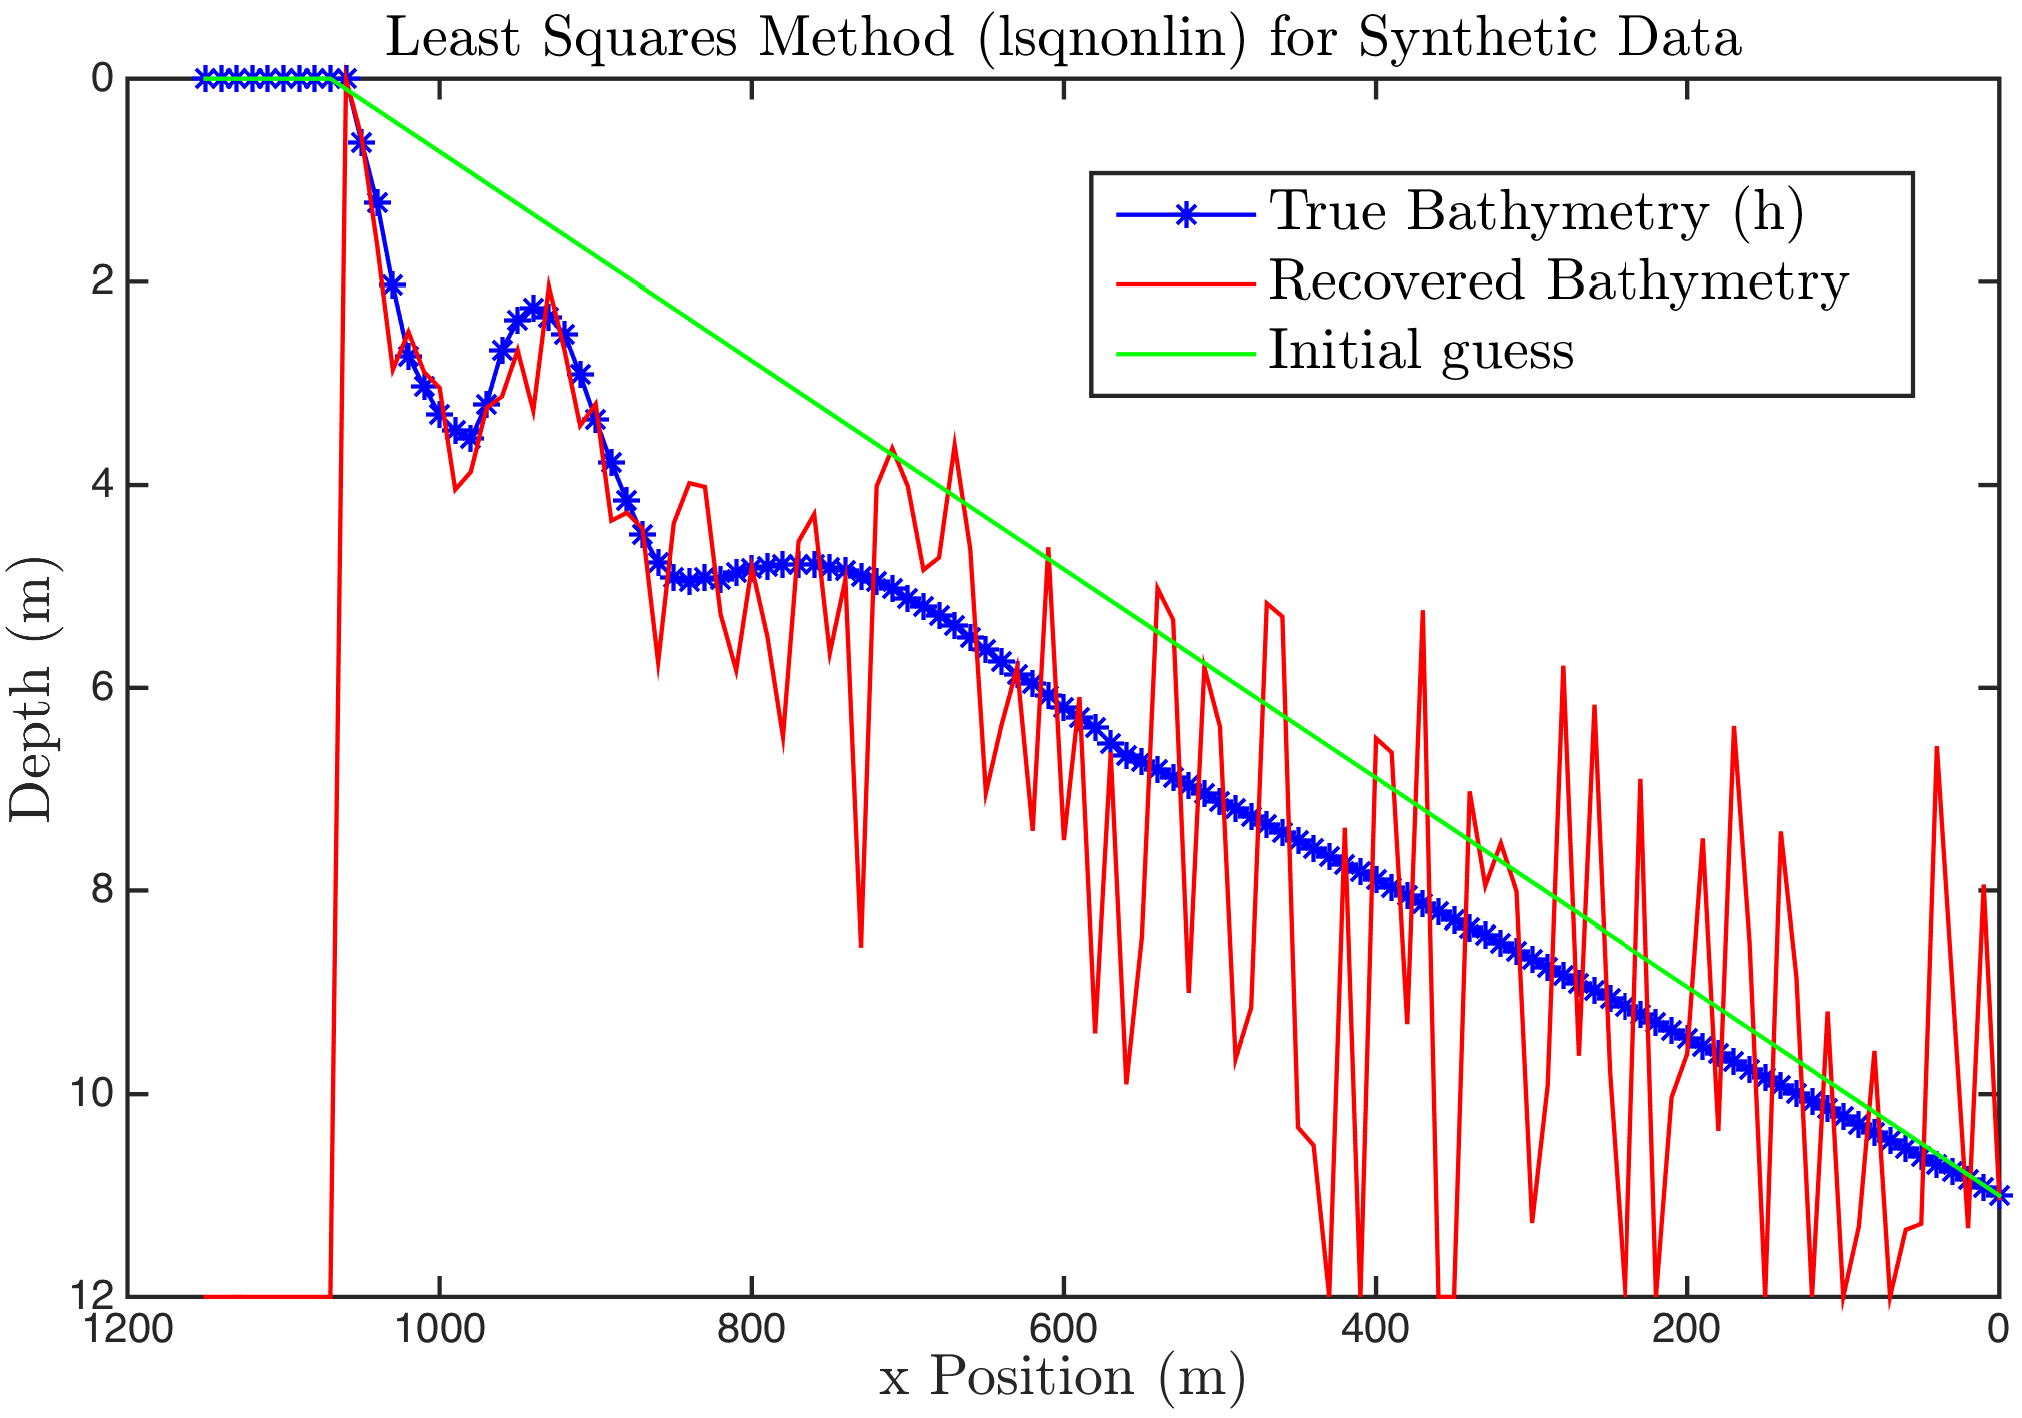
\includegraphics[scale=0.6]{img/lsqnonlin_simulated_10m.png} %plot20 
\caption{lsqnonlin method reconstruction of depth $\mathbf{h}$ using the simulated data.}
\label{fmincon_simulated}
\end{figure}

\begin{figure}[H]
\center
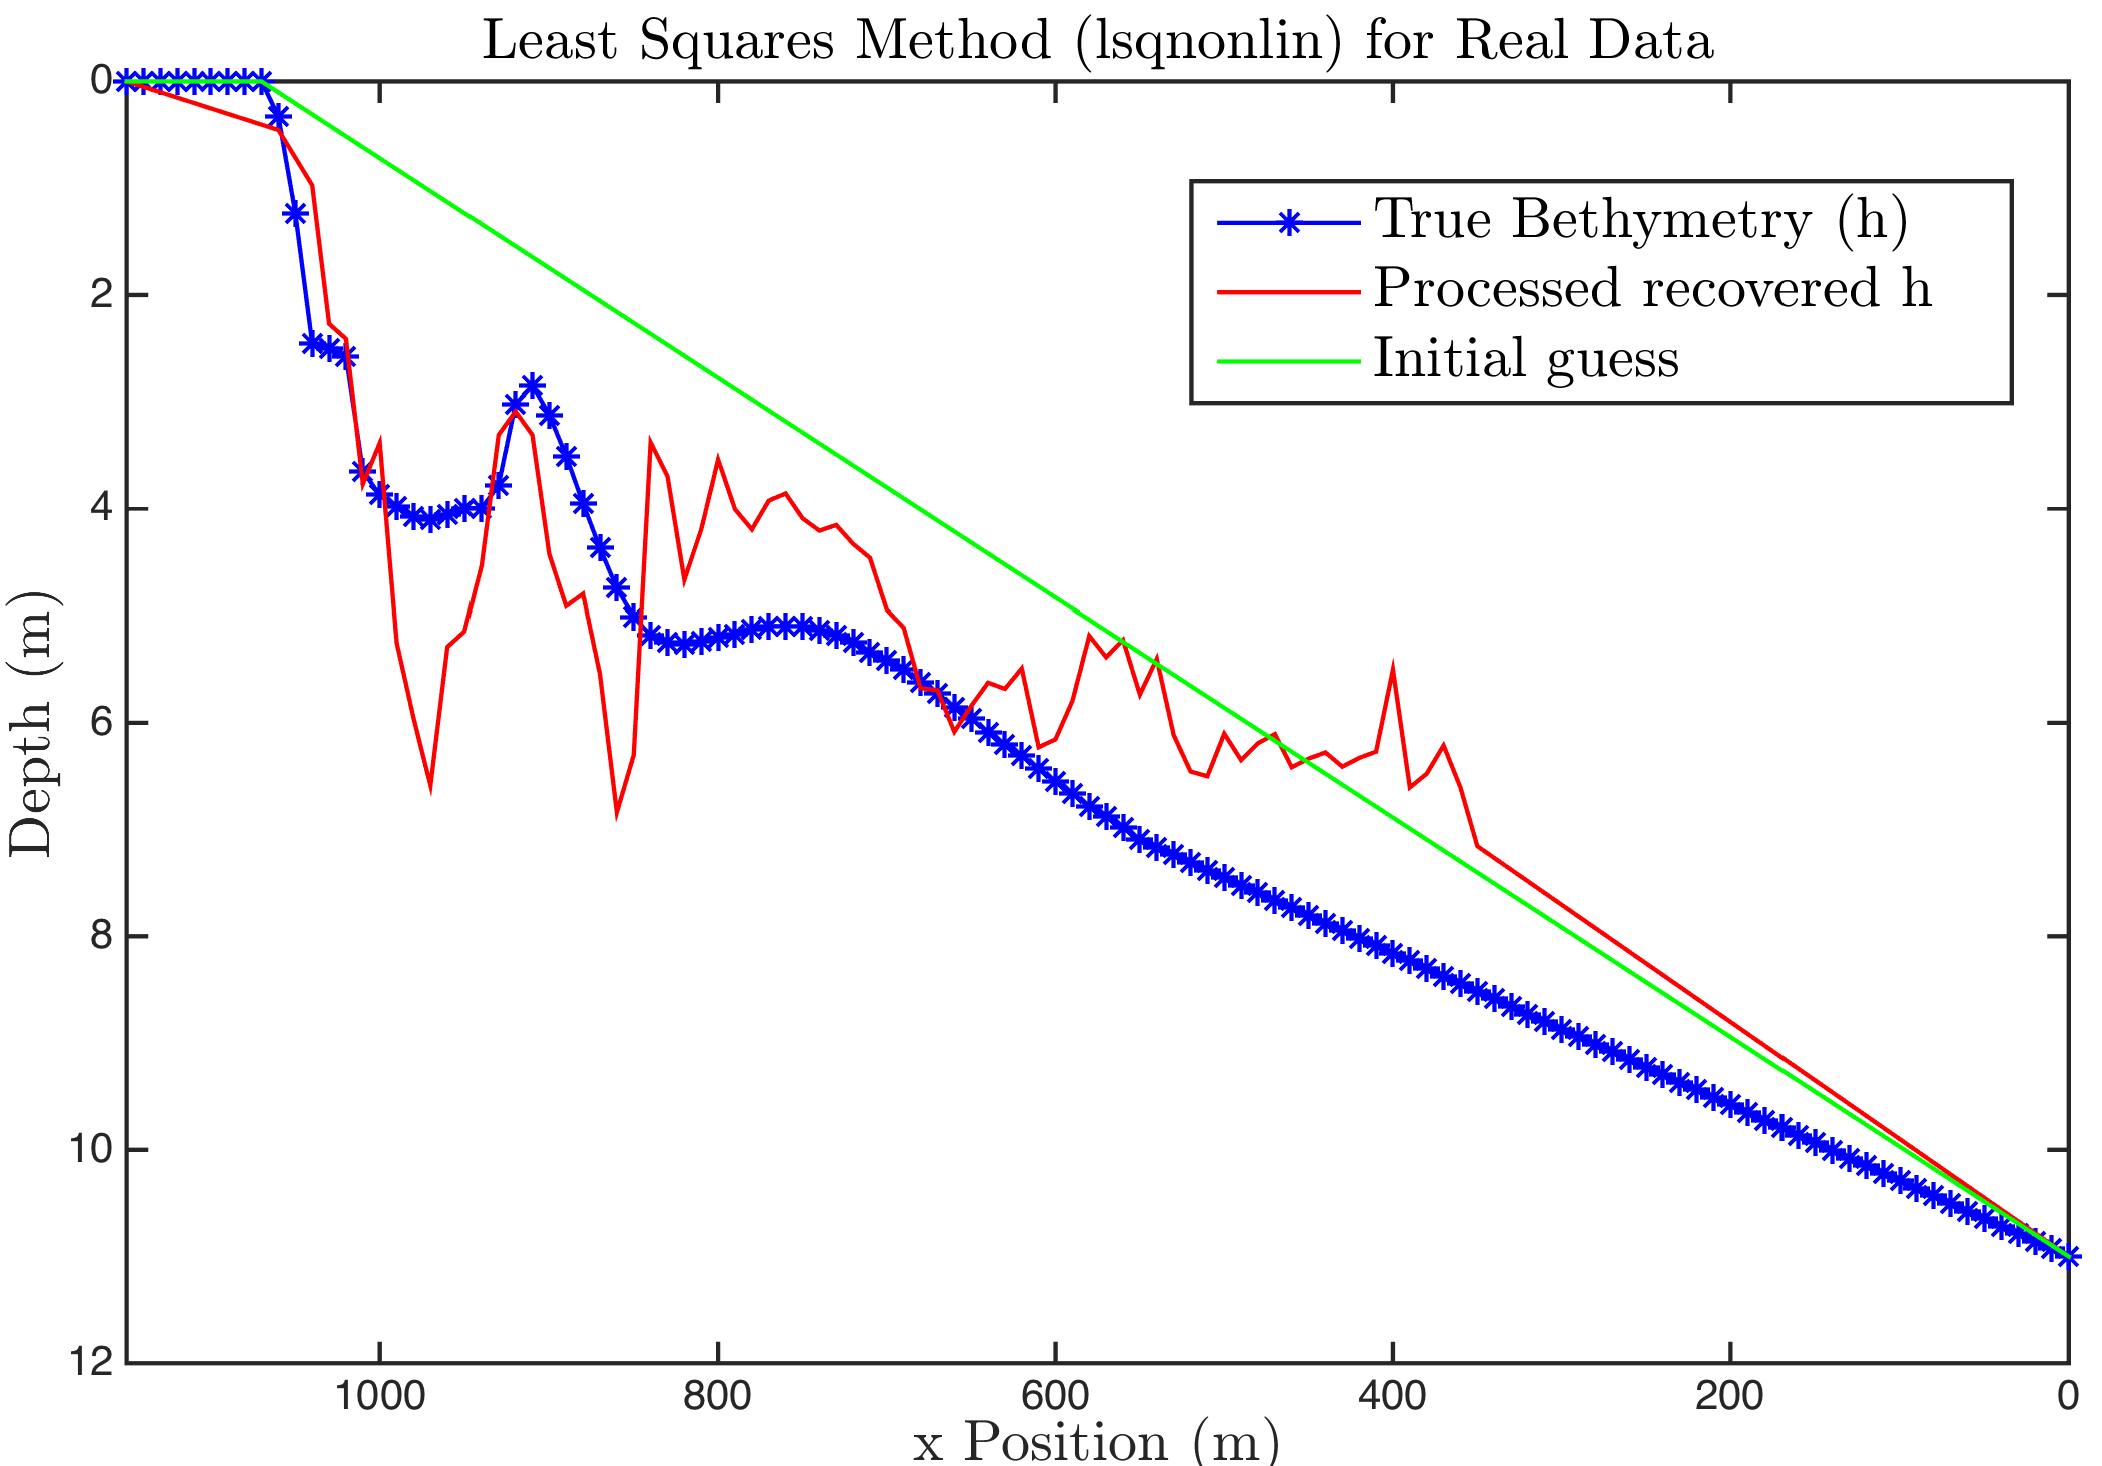
\includegraphics[scale=0.6]{img/lsqnonlin_real_data_oct09.png} %plot20 
\caption{lsqnonlin method reconstruction of depth $\mathbf{h}$ using the simulated data.}
\label{fmincon_simulated}
\end{figure}

\subsection{Tikhonov Regularization}

\begin{equation}\label{LS-regBC}
\mathbf{\hat{h}} = \underset{\mathbf{0} \preceq \mathbf{h} \preceq \mathbf{11}}{\arg \min} \ \ \|  \mathbf{A}(\mathbf{h}) -  \mathbf{d} \|_2^2  +  \alpha \| \mathbf{h}\|_2^2,
\end{equation}

[Using the Matlab's fmincon function ]


\begin{figure}[H]
\center
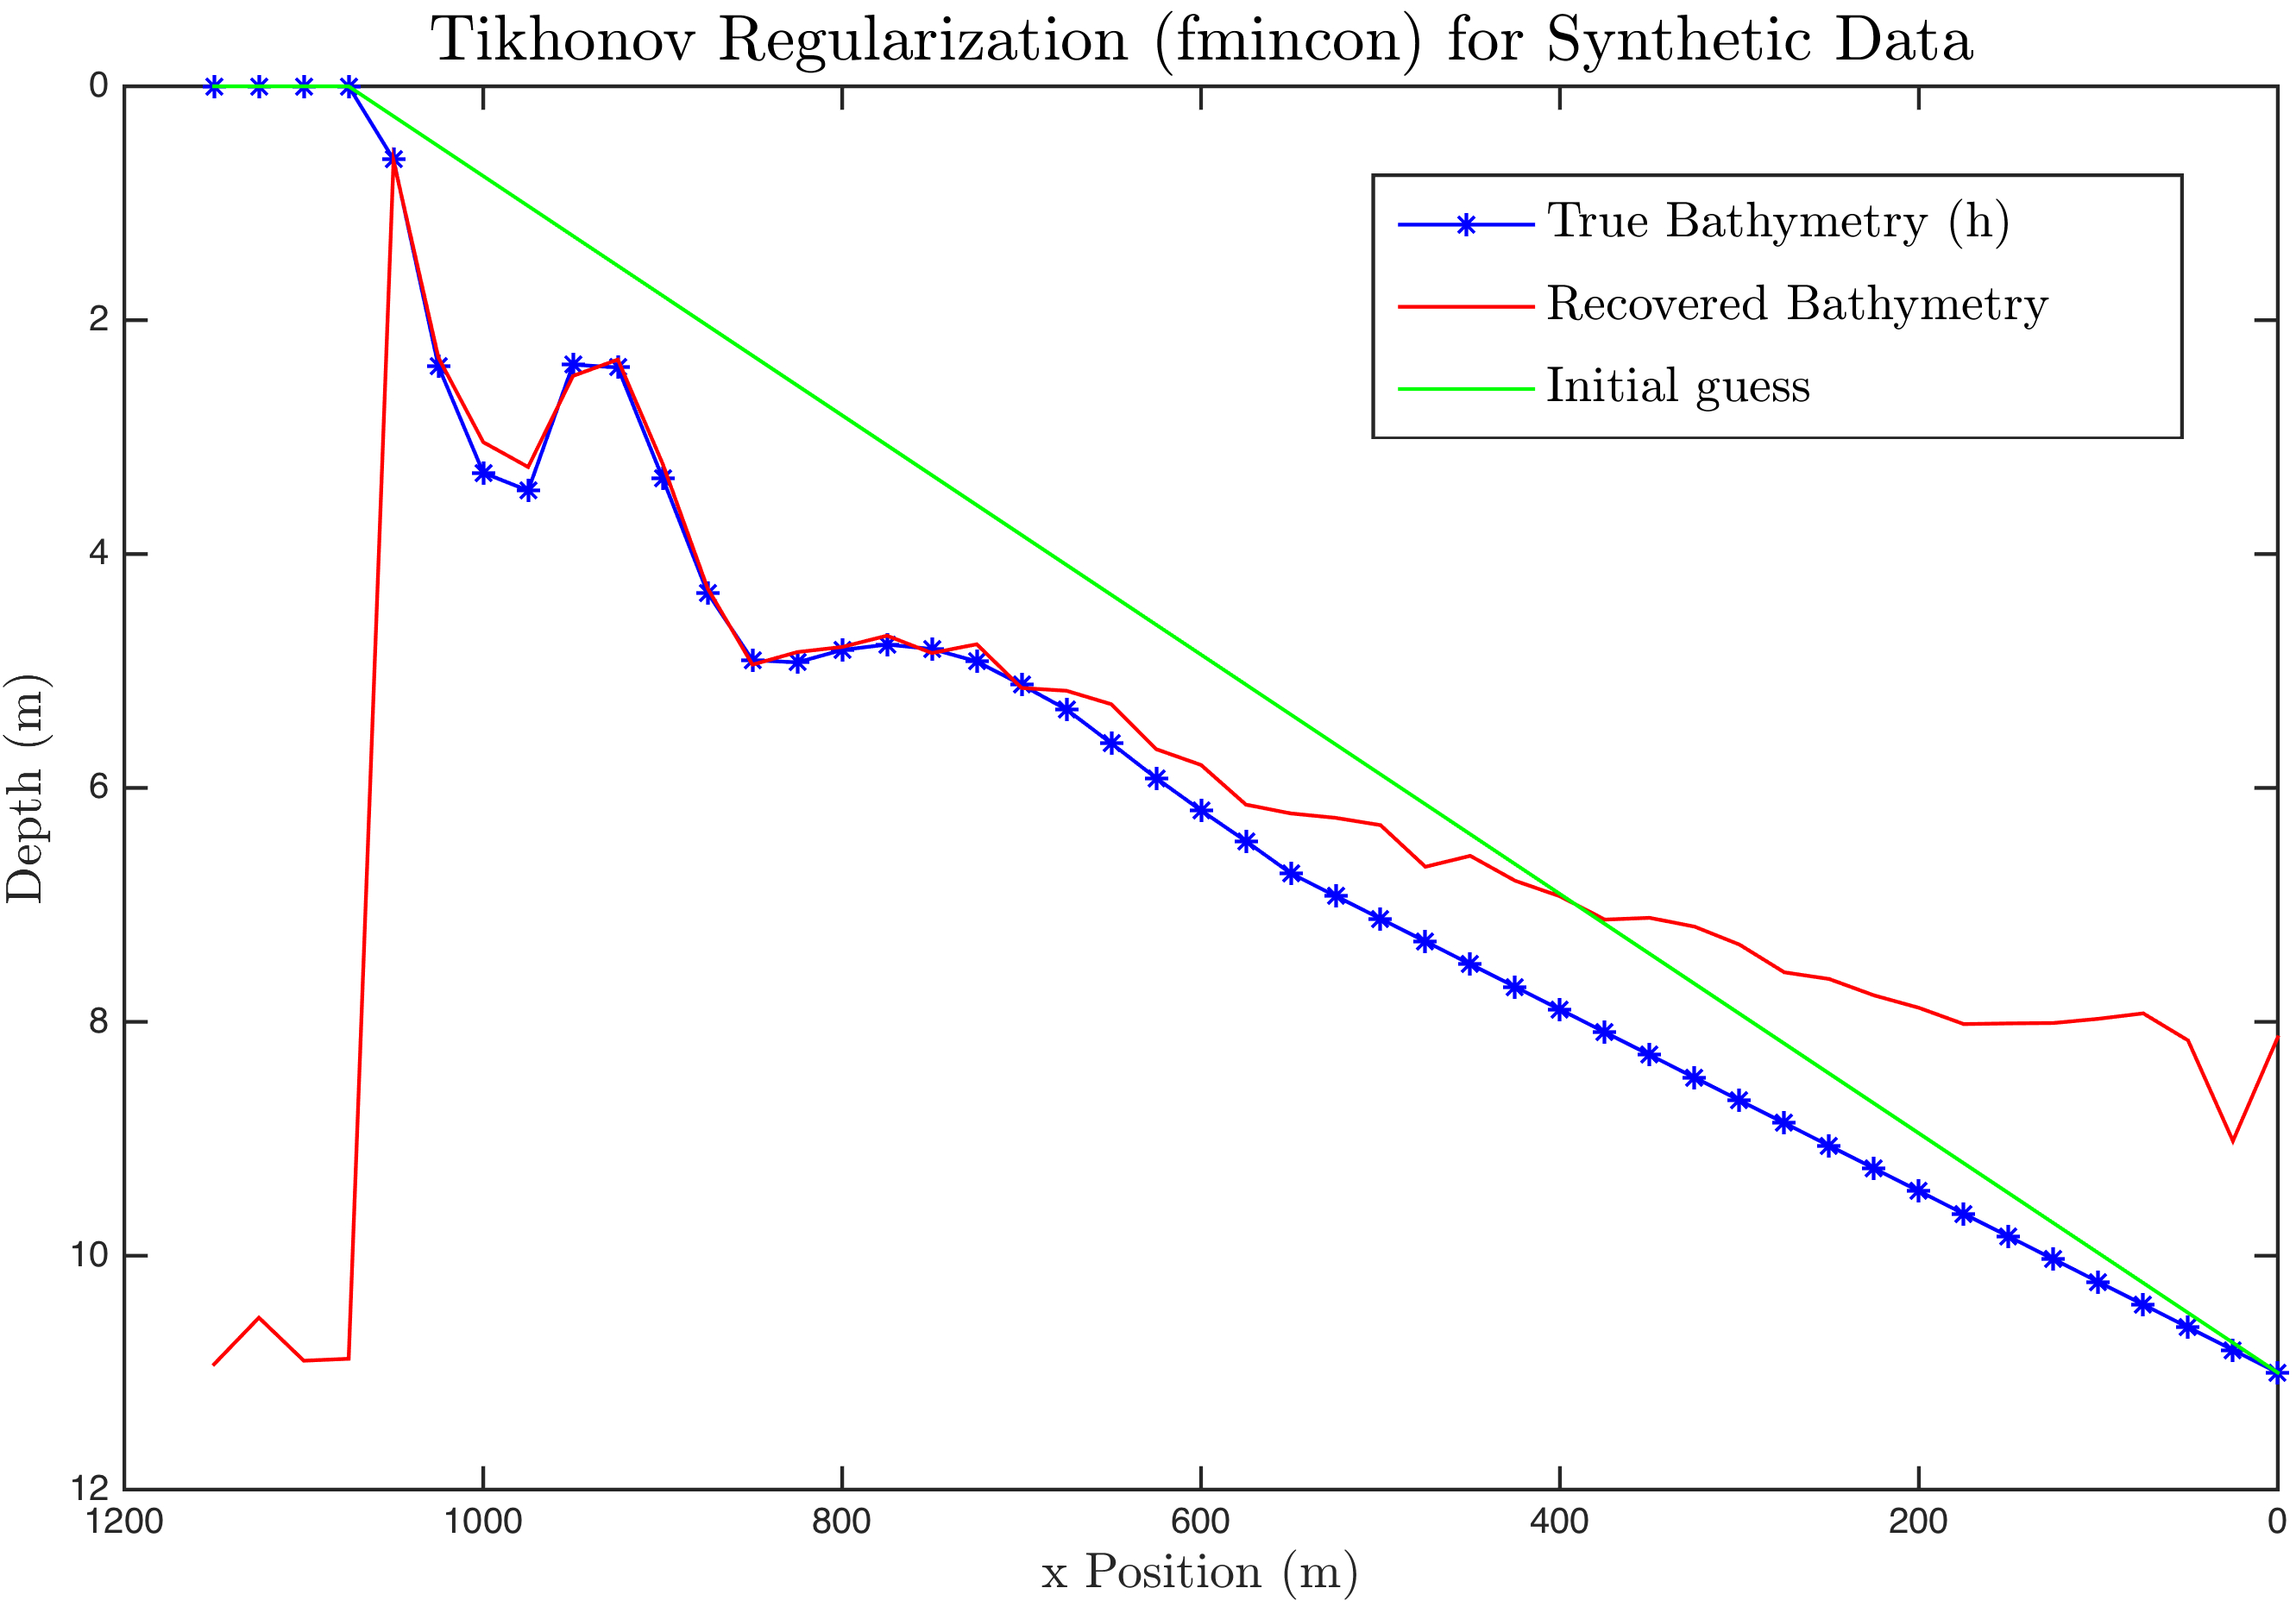
\includegraphics[scale=0.46]{img/fmincon_simulated_25m.png} %plot20 
\caption{fmincon method reconstruction of depth $\mathbf{h}$ using the simulated data.}
\label{fmincon_simulated}
\end{figure}

\begin{figure}[H]
\center
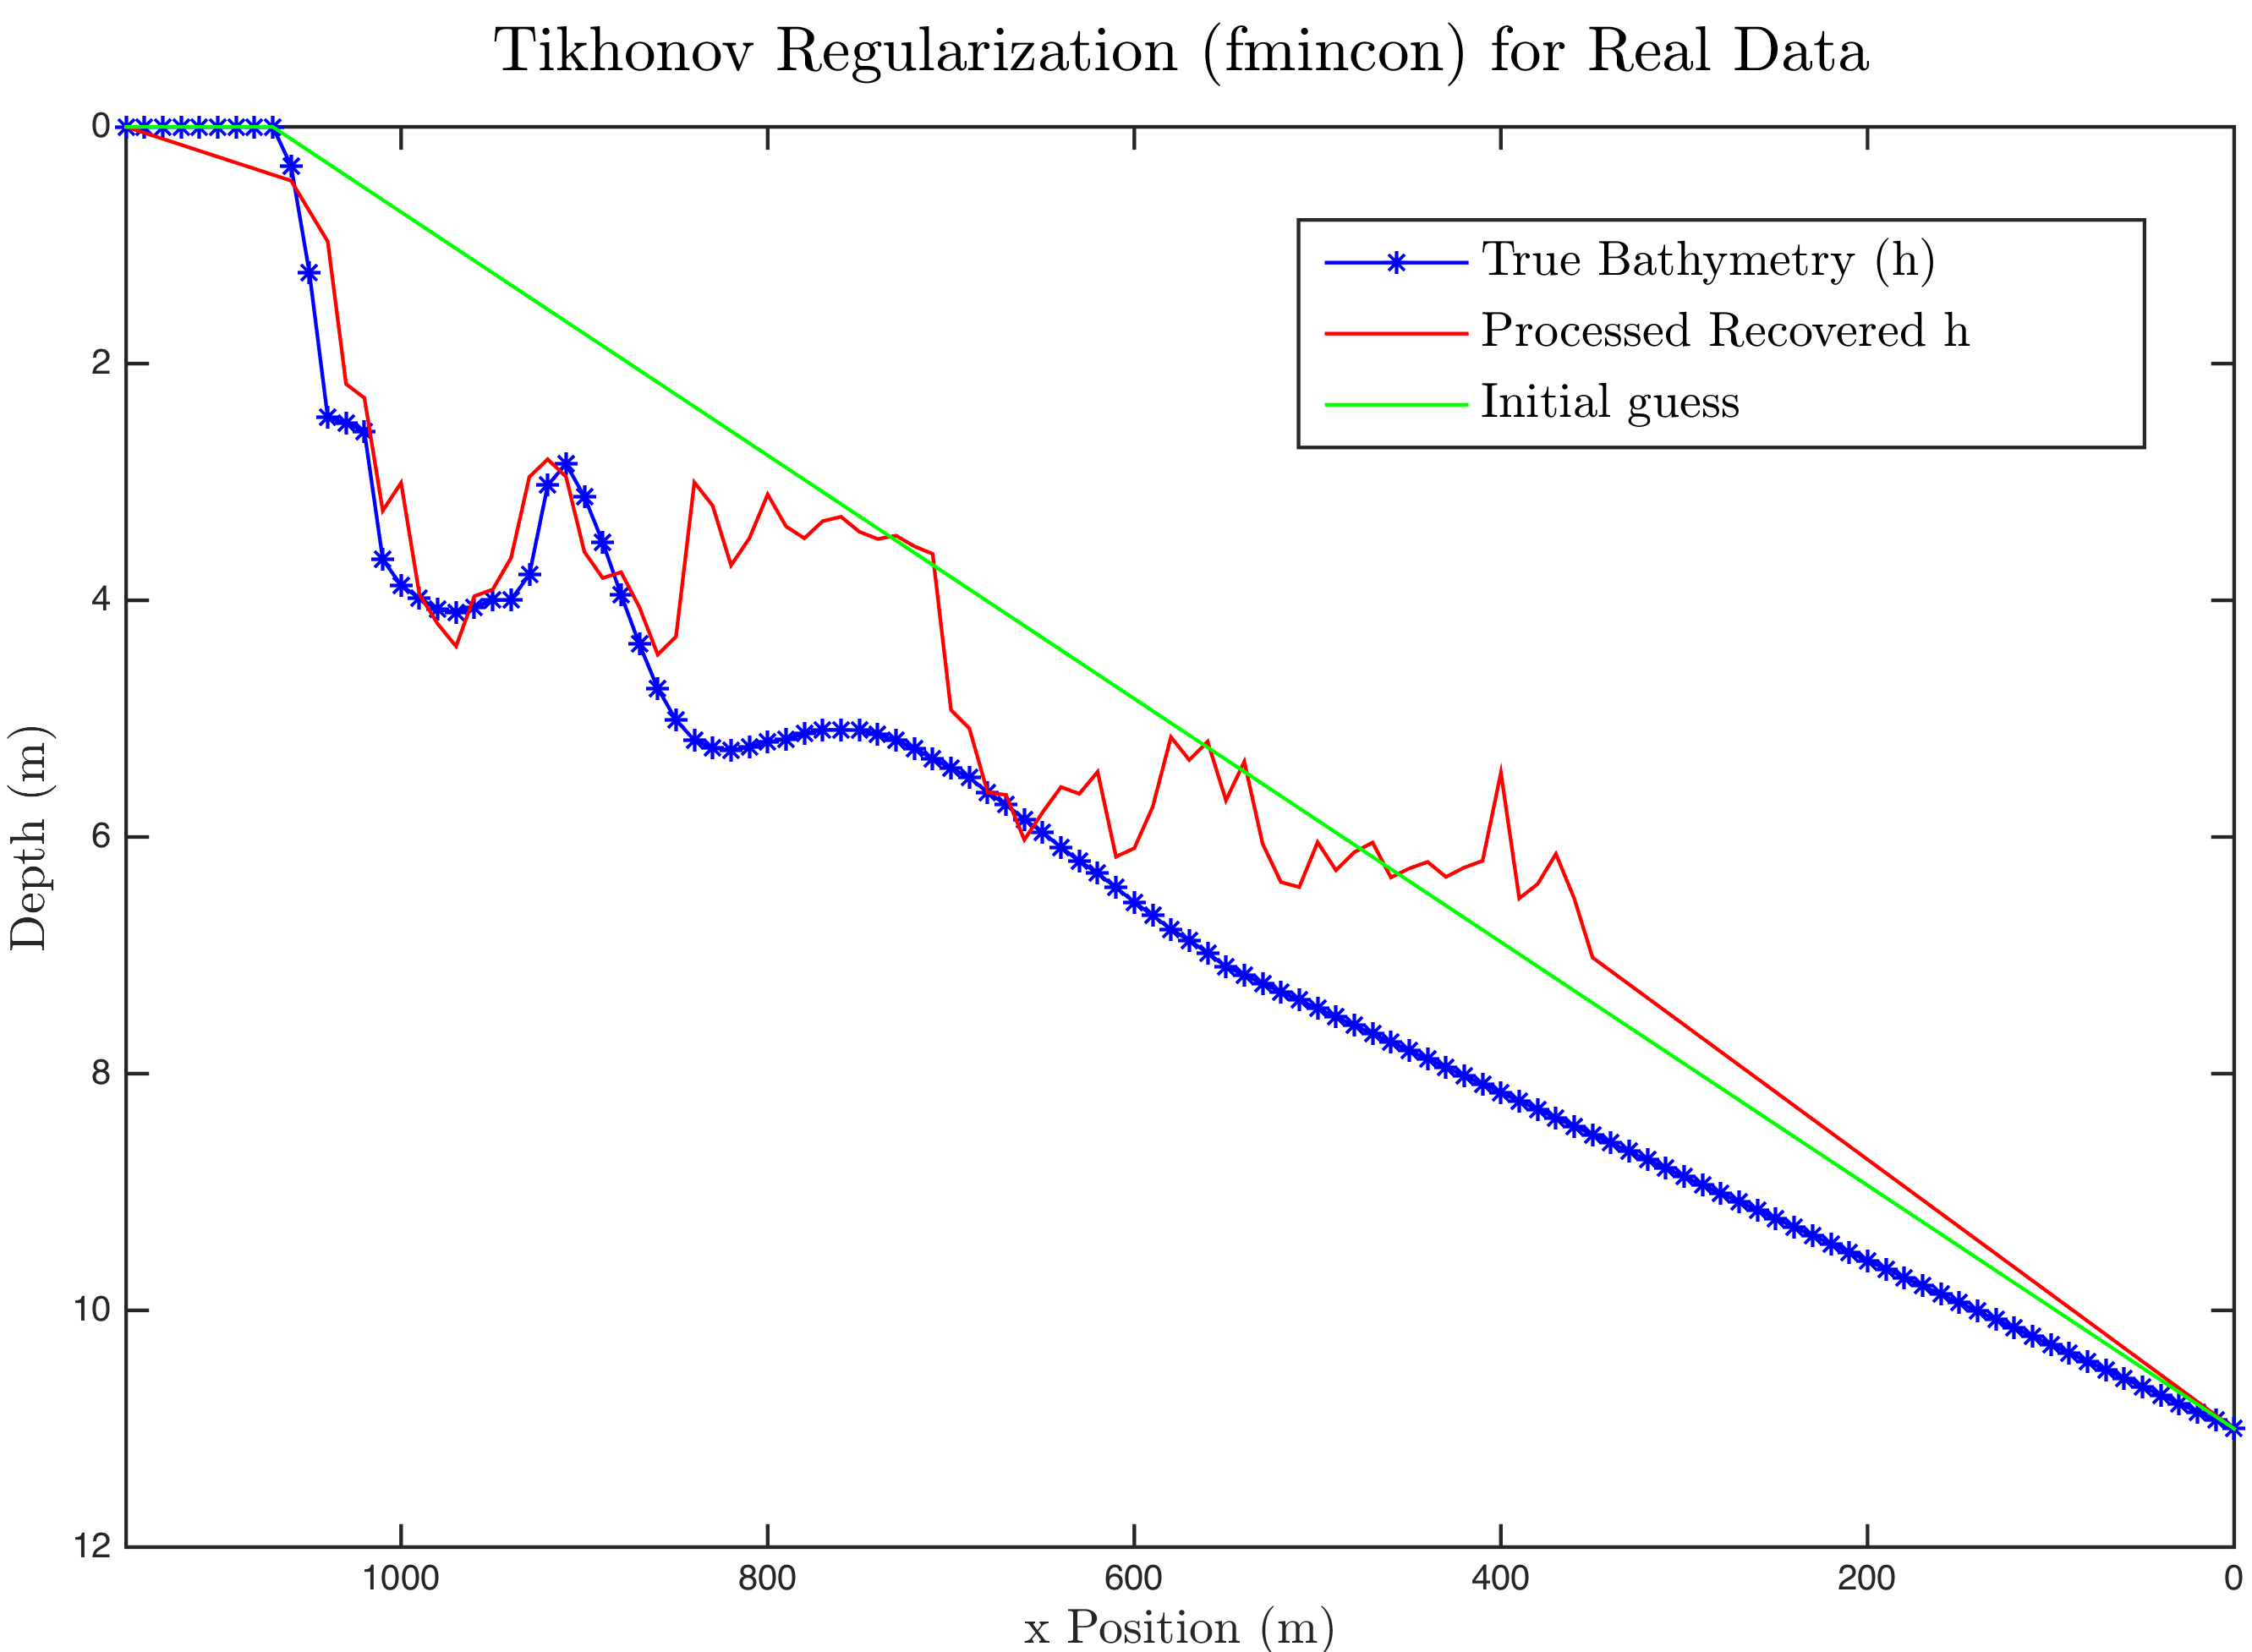
\includegraphics[scale=0.46]{img/fmincon_real_data_oct09.png} %plot20 
\caption{fmincon method reconstruction of depth $\mathbf{h}$ using the simulated data.}
\label{fmincon_simulated}
\end{figure}




\subsection{Bayesian Inference}
The Bayesian inversion approach samples a posterior distribution of depth profiles. For comparison to the other inversion methods, we consider only the depth at each grid point which corresponds to the maximum of the posterior probability distribution at that point. This is achieved by taking the maximum of the kernel density of the estimated depth distribution at each point along the 1D profile. 

This method is first applied using synthetic $k$ input and the resulting depth estimate is shown in Figure~\ref{mcmc-synthetic}. As for other methods, the synthetic result accurately represents the sandbar located at $x~\sim~950~m$ along the profile, which is an important feature to recreate. However, at offshore locations ($x~<~600~m$), the estimation appears to break down. As in other methods, this is expected because of the lower sensitivity of $k$ on $h$ at these depths, a relationship on which our inverse methods rely.


\begin{figure}[H]
\center
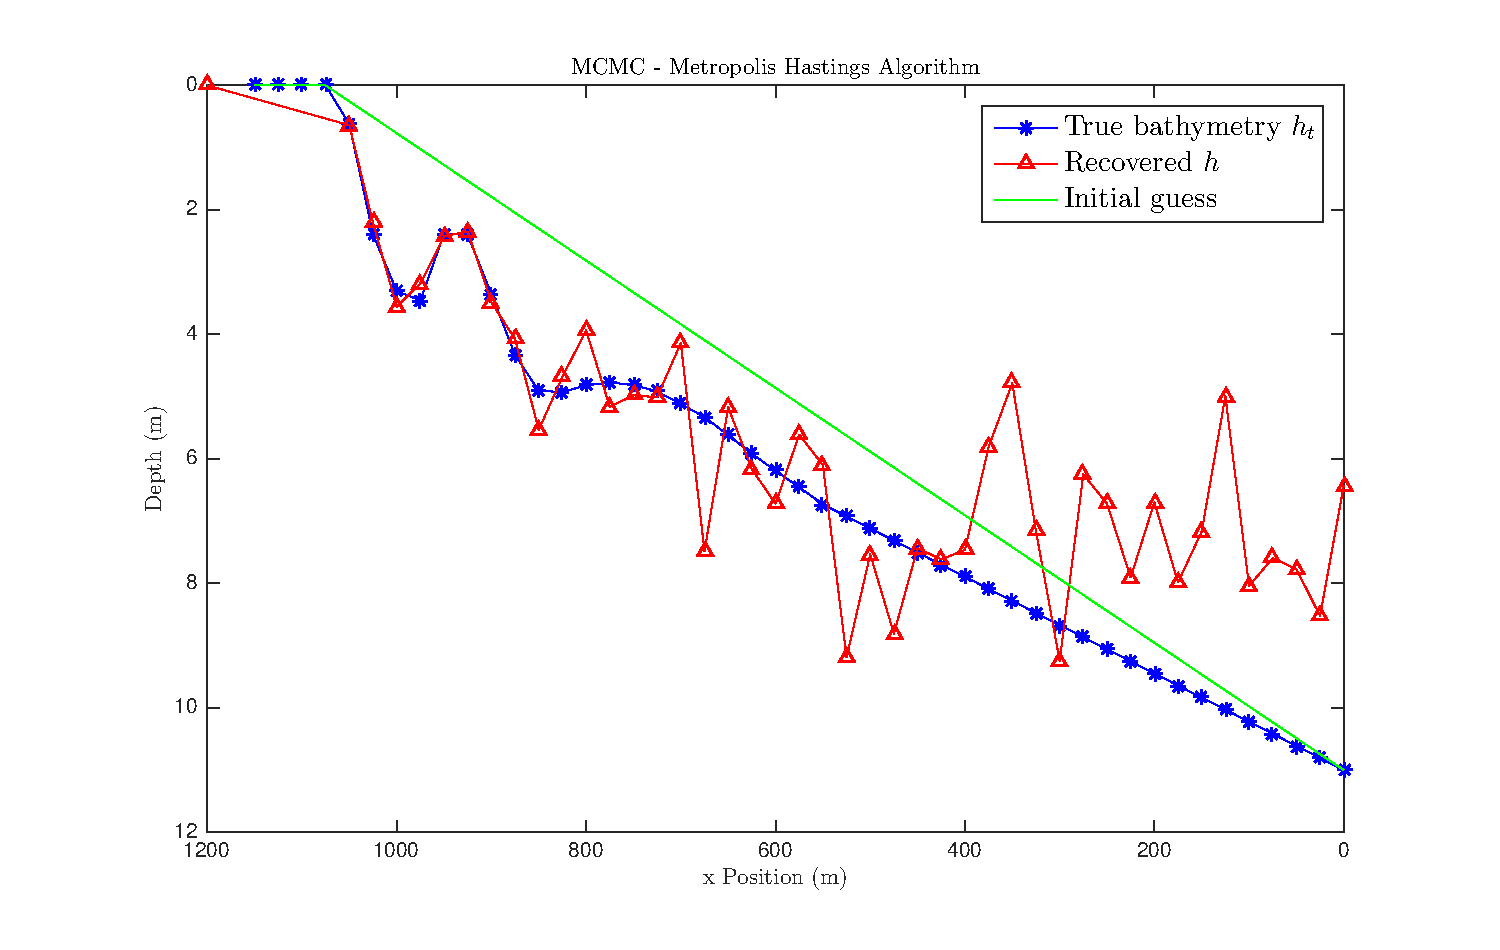
\includegraphics[scale=0.46]{img/MCMC-manufactured.eps} %plot20 
\caption{Bathymetry estimate from the Bayesian Markov Chain Monte Carlo approach. The initial $h$ guess is shown in green, the true $h$ is shown in blue, and the derived estimate of $h$ is shown in red.}
\label{mcmc-synthetic}
\end{figure}

Real $k$ data is then used to estimate the same bathymetry profile (Figure~\ref{mcmc-real}). We find...


Unlike the other methods, the Bayesian approach results in a distribution of depth profiles which optimize $h$ given uncertain $k$. Measurements of wave number, $k$, are not perfect and our resulting distribution of depth profiles translates that uncertainty binto an ensemble of depth estimates which are consistent with the $k$ data to within uncertainty. Figures~\ref{mcmc-posterior-h-synthetic} and \ref{mcmc-posterior-h-real} show the resulting posterior depth distributions. Note that...





%\subsection{Estimating Bathymetry using Real Data}

\section{Computational Experiments}
Give enough details so that readers can duplicate your experiments.

\begin{itemize}
\item Describe the precise purpose of the experiments, and what they 
are supposed to show.

\item Describe and justify your test data, and any assumptions you made to 
simplify the problem.

\item Describe the software you used, and the 
parameter values you selected.

\item 
For every figure, describe the meaning and units of the coordinate axes, 
and what is being plotted.

\item Describe the conclusions you can draw from your experiments
\end{itemize}

\section{Summary and Future Work}
[Need to solve the following problem with priors $\mathbf{h}_p$].

\begin{equation}\label{LS-regBC}
\mathbf{\hat{h}} = \underset{\mathbf{0} \preceq \mathbf{h} \preceq \mathbf{11}}{\arg \min} \ \ \|  \mathbf{A}(\mathbf{h}) -  \mathbf{d} \|_2^2  +  \alpha \| \mathbf{h} -  \mathbf{h}_p\|_2^2,
\end{equation}

[Want to use proper method to find the optimum regularization parameter $\alpha$]


\begin{itemize}
\item Briefly summarize your contributions, and their possible
impact on the field (but don't just repeat the abstract or introduction).
\item Identify the limitations of your approach.
\item Suggest improvements for future work.
\item Outline open problems.
\end{itemize}

\bibliography{bib}

\end{document}
